% !TeX encoding = UTF-8
\documentclass[twoside,english,1p,final,sort&compress]{elsarticle}
\usepackage[T1]{fontenc}
\usepackage[utf8]{inputenc}
\pagestyle{headings}
\usepackage{amsthm}
%\usepackage{gensymb}
\usepackage{xspace}
\usepackage{amsmath}
\usepackage{accents}
\usepackage{multirow}
\usepackage{arydshln}
\usepackage{xcolor}
\usepackage{amssymb}
\usepackage{subcaption}
\usepackage{adjustbox}
\usepackage{placeins}
\usepackage[colorlinks = true]{hyperref}

% To have Times only in text not maths
\renewcommand{\rmdefault}{ptm}

\makeatletter

\theoremstyle{plain}
\newtheorem{thm}{\protect\theoremname}

% specify here the journal
\journal{International Journal of Mechanical Sciences}

% use this if you need line numbers
\usepackage{lineno}

\makeatother

\usepackage{babel}
\providecommand{\theoremname}{Theorem}

\newcommand{\dotp}{\boldsymbol{\cdot}}
%\newcommand{\ccirc}{\kern0.5ex\vcenter{\hbox{$\scriptstyle\circ$}}\kern0.5ex}
\newcommand{\e}[1]{\exp\left({#1}\right)}
\newcommand{\lay}[1]{^{(#1)}}
\newcommand{\mdot}[1]{\accentset{\mbox{\bfseries .}}{#1}}
\newcommand*{\ie}{\emph{i.e.}\@\xspace}
\newcommand*{\versus}{\emph{vs.}\@\xspace}
\newcommand*{\eal}{et \emph{al.}\@\xspace}
\newcommand*{\eg}{e.g.,\@\xspace}
\newcommand{\RMSE}{\text{E}_\text{RMS}}
\newcommand{\AARE}{\text{E}_\text{AAR}}
\newcommand{\R}{\text{R}}
%\newcommand{\Dev}	{\mbox{\Large\ensuremath{\mathsf{s}}}}
%\DeclareMathOperator{\sech}{sech}
%\DeclareMathOperator{\sigmoid}{sig}

\usepackage{esvect}
% Redefine the esvector shape to remove overlapping
\def\traitfill@#1#2#3#4{%
  $\m@th\mkern2mu\relax#4#1\mkern-1.5mu %on met \relbaredd au d\'ebut
   \cleaders\hbox{$#4\mkern-0.3mu#2\mkern-0.3mu$}\hfill %remplit avec relbareda
   \mkern-1.5mu#3$%
}
\renewcommand{\overrightarrow}{\vv}

% This is used to add comments into the text
\usepackage{soul} %Can also be used to highlight text with \hl{highlighted text}
\usepackage{color}
\definecolor{VWyellow}{RGB}{255,251,150} % VaporWave color palette
\DeclareRobustCommand{\OP}[1]{ {\begingroup\sethlcolor{VWyellow}\textcolor{red}{\hl{\textbf{Olivier Pantal\'e:}#1}}\endgroup} }

\begin{document}
\begin{frontmatter}

\title{Compararison of analytical and artificial neural network models in predicting hot deformation behavior of AISI P20 and  interpolation-extrapolation capacity validation}

\author[LGP]{Pierre Tize Mha}
\author[ETS]{Prashant Dhondapure}
\author[LGP]{Amèvi Tongne}
\author[ETS]{Mohammad Jahazi}
\author[LGP]{Olivier Pantalé \corref{cor1}}
\ead{Olivier.Pantale@enit.fr}
\ead[url]{http://www.enit.fr}

\cortext[cor1]{Corresponding author}

\address[LGP]{Laboratoire Génie de Production, INP/ENIT, Université de Toulouse, 47 Av d'Azereix, Tarbes, France 65016}
\address[ETS]{École de Technologie Supérieure, 1100 Rue Notre Dame O, Montréal, QC H3C 1K3}

\begin{abstract}
The high-temperature deformation behavior of the AISI P20 alloy was investigated by performing hot compression tests over a wide range of strains ($0.025 - 0.7$),  strain rates ($0.001\ \text{s}^{-1} - 5\ \text{s}^{-1}$) and temperatures ($1050\text{°C}-1250\text{°C}$). Based on the experimental data (stress-strain curves), empirical models as the Johnson-Cook (JC), Modified-Zerilli-Armstrong (MZA), Hansel-Spittel (HS), Arhenius (AR) and PTM on the one hand and an ANN model on the other hand were developed to predict the flow behavior of this alloy. Then, a comparative study between the analytical models and the ANN model was carried out on the basis of the calculation of some coefficients allowing to test the efficiency of each model. These coefficients are the correlation coefficient $R$, the Average Absolute  Relative Error $\AARE$ and the Root Mean Square Error ($\RMSE$). From these parameters it was found that the JC, MZA and HS models are not suitable for predicting the behavior of AISI P20 alloy whereas the AR and PTM models can be used for most strain rates to predict the flow behavior of this alloy. For the strain rate ($\mdot\varepsilon^p = 0.01\ \text{s}^{-1}$)  the AR model fails to describe the flow for temperatures $1050$°C and $1100$°C  while in the case of the PTM model, the strain rate  ($\mdot\varepsilon^p = 0.1\ \text{s}^{-1}$) is not well described. This is due to the fact that this model is a sequence of polynomials which can create oscillations if the degree is high. Regarding the ANN model, the architecture retained is composed of two hidden layers of which the first hidden layer contains $15$ neurons and the second contains $7$ neurons and the input layer contains $3$ neurons corresponding to the strain ($\varepsilon^p$), strain rate ($\mdot\varepsilon^p$) and temperature ($T$) and the output layer contains a single neuron corresponding to the flow stress ($\sigma^y$). The results of the ANN model show a very good agreement between the predictions and the experiment. This demonstrates that this  formulation of constitutive law exceeds highly the analytical models in terms of prediction. To validate the performance of these models their capacities to interpolate and extrapolate the data were also tested where all the models relatively prove a good interpolation capacity whereas this is not the case for extrapolation where only the AR, PTM and ANN models are acceptable but still mentioning that the ANN model remains the best in both interpolation and extrapolation.
\end{abstract}

\begin{keyword}
Zerilli-Armstrong flow law \sep Constitutive behavior \sep Arhenius flow law \sep Hansel-Spittel flow law \sep Johnson-Cook flow law \sep interpolation \sep extrapolation \sep Artificial neural network
\end{keyword}

\end{frontmatter}
\linenumbers

%--------------------------------------------------------------------------
\section{Introduction\label{sec:Introduction}}
%--------------------------------------------------------------------------
Continuous casting and rolling techniques are an integral part of material forming methods. Advantages of this method include increased process efficiency, energy savings, improved casting quality and easier mechanization and automation. Deformation, a complex process involving simultaneous elastic and plastic deformation, is accompanied by high temperatures, high strain rates, and complex and variable frictional conditions \cite{He-2013}, for which, analytical methods are not available for quantitative study and analysis of the deformation mechanism. On the other hand, conducting experimental tests is not only time-consuming but also requires a high financial investment \cite{Changizian-2012}. As an alternative approach to the previous two, the Finite Element Method (FEM) is widely used as a tool for analysis and optimization of process parameters in the processing of various materials. Finite element modeling effectively compensates for the shortcomings of analytical and experimental methods and is playing an increasingly important role in determining process parameters, improving product quality, and gaining in-depth knowledge of deformation mechanisms. For example, FEM has been widely used to simulate and analyze hot forming processes of steel, such as forging, rolling, extrusion and casting, but the quality of the numerical solution provided by this method is highly dependent on the constitutive equation of the modeled material \cite{Qin-2010, Mandal-2009, Ji-2018}.

Hot forming processes are an essential step in the manufacture of mechanical components and directly affect the final quality of the products through their strong influence on the micro-structure and mechanical properties \cite{Ashtiani-2012}. Several metallurgical phenomena such as work hardening and dynamic softening (dynamic recovery and re-crystallization), which very often occur during hot working, influence the behavior and deformation of materials. The complexity of the thermomechanical behavior usually leads to the fact that it can only be taken into account accurately by using a numerical approach to obtain the response of the material under the specified loading conditions. To this end, a mathematical formulation is typically used to represent the flow of a material in a form that can be used in finite element software \cite{Lin-2008-P, Wu-2012}.

For several years, many researchers have developed methods to predict the thermomechanical behavior of materials under hot working conditions using constitutive models. Thus, various forms of constitutive equations have been proposed to describe the flow of materials, among which, phenomenological, semi-empirical, physical models or models based on Artificial Neural Networks (ANN) \cite{Lin-2011, Shin-2010, Rusinek-2010, Pantale-2021}. Among the large number of models available in the literature, the Johnson-Cook (JC) \cite{Johnson-1983, Johnson-1985} and Zerilli-Armstrong (ZA) \cite{Zerilli-1987} models are the best known and most widely available in finite element codes. The Johnson-Cook model is the most widely used because it is simple to identify and use and has few parameters to determine \cite{Khan-2004, NematNasser-2003}. However, this model, in its original state, has some shortcomings related to nonlinear coupling phenomena not taken into account in the material behavior. We refer here to strain hardening, strain rate hardening and thermal effects that are taken into account in a non-coupled manner in the JC model as analyzed by Jia \eal \cite{Jia-2021}. To circumvent these shortcomings, several modified forms of the Johnson-Cook model have been developed in the past \cite{Rule-1998, Vural-2003, Lin-2010, Lin-2012, Li-2013, Zhou-2019, Zhang-2015}. Due to its more physics-based formulation, the ZA model is often preferred to the JC model because it allows the coupling of strain rate and temperature effects \cite{Johnson-1988, Voyiadjis-2005, Dey-2007}. However, this model has other drawbacks related to the limit value of the test temperature. Indeed, this model applies only to low strain rates and for temperatures limited to about 60~\% of $T_m$ (where $T_m$ is the melting temperature of the material) \cite{Chiou-2005, Lee-2005, Chen-2007, Lee-2006}. Moreover, this model, in its original form, does not take into account the coupling between deformation and temperature effects \cite{Samantaray-2009}. In order to reduce these shortcomings (and to apply this model to a wider range of temperatures) of the ZA model, modified forms of Zerilli-Armstrong (MZA) have been proposed by several authors in recent years \cite{NematNasser-2004, Lennon-2004, Muralli-2017, Cheng-2021, Muralli-2021}.

The Arrhenius-type hyperbolic sine constitutive model is one of the most widely used phenomenological models both for the prediction of the hot deformation behavior of materials and for the analysis of the micro-structure of the material under study because this model allows the estimation of the deformation energy of the material \cite{Jonas-1969, Zhang-2012, Mostafaei-2012}. Its original formulation has been revised several times to correctly describe the resulting experimental behavior. In order to increase the accuracy of the model, the effects of strain \cite{Slooff-2007, Li-2012, Xu-2013}, strain rate \cite{Lin-2008-C, Mandal-2009} have been considered by several authors. For example, Sloof \eal \cite{Slooff-2007} introduced a strain-dependent parameter into the initial formulation of the Arhenius model so that his model could predict the high-temperature flow of a magnesium alloy. Lin \eal \cite{Lin-2008-C}, on the other hand, modified the model by introducing a strain rate compensation factor.

Users of the Forge software make extensive use of the model developed by Hansel and Spittel \cite{Hensel-1978}, commonly referred to as the HS model, which is a thermo-visco-plastic model whose formulation is based on a product of functions dependent on the three physical variables.  Unlike the JC model, this formulation is based on parameters that are determined simultaneously. This model is simple to use and has $8$ parameters that are easy to determine. The limitation of this model is its loss of accuracy in some cases when the $8$ parameters are defined. This is why many works often limit its identification to only $5$ or $6$ parameters. This has been verified in our study where the smallest error of the model is obtained with only $5$ parameters identified.

The fixed and limited number of parameters imposed by each analytical model as presented above has both advantages and disadvantages. These models have few parameters and are therefore easy to identify, but when these models have to be applied to a material different from the one for which they were initially developed they lose their performance as in the case of the HS model. To try to solve this problem, Tize Mha \eal \cite{TizeMha-2022} has proposed a formulation where the number of parameters is not known in advance. The idea is to make the formulation of an analytical model flexible so that it can be adapted to many materials. This formulation is based on the MZA model and polynomial functions of undefined order are used in the identification phase. 

Behavior modeling based on an artificial neural network is an approach to predict the flow of materials without requiring a mathematical formulation of the flow law. It is therefore not necessary to postulate a mathematical expression to identify the parameters of the model. Since the behavior of materials is highly nonlinear at high temperatures, and depends on many factors that are also nonlinear, the evaluation of the flow stress by an analytical model whose parameters are identified by a classical regression method is limited. Faced with these limitations, ANN models are of major interest because they are particularly suited to deal with complex and nonlinear relationships. Consequently, ANNs have been successfully applied to predict the flow of materials under hot working conditions \cite{Lin-2008-ANN, Lu-2011-ANN, Ashtiani-2016-CSP, Stoffel-2019-NNB, Pantale-2021}. They provide a fundamentally different approach to statistical or numerical techniques for modeling materials.

In this work, the high-temperature thermomechanical behavior of AISI P20 modified carbon steel subjected to compression tests in a Gleeble thermomechanical simulator was studied. From the experimental data obtained from the compression tests, five analytical models were identified in order to select the one that best describes the behavior of this alloy. A flow model based on an artificial neural network was also developed and identified, and a comparative study between the five analytical models and the ANN model is proposed. A fundamental concern addressed in this work is the ability of a model to interpolate and extrapolate the results of the model with respect to the range of conditions covered by the experimental tests.

The main parts of this work are as follows: Section \ref{sec:Materials} presents the hardware (Gleeble thermomechanical simulator), the experimental procedure, the material and the results of the compression tests performed for this study. Section \ref{sec:ConstLaws} is devoted to the presentation of the five analytical models, the ANN model, the identification of their parameters and the comparison of the performances of these models. Section \ref{sec:inExtrapolation} details the interpolation and extrapolation capabilities of each model proposed in this paper. Conclusions and future work are detailed in Section \ref{sec:Conclusion}.

%----------------------------------------------
\section{Materials and Experiments\label{sec:Materials}}
%----------------------------------------------

%----------------------------------------------
\subsection{Experimental procedure}
%----------------------------------------------

The material used in this study is the modified carbon alloy AISI P20 whose chemical composition is given in Table \ref{tab:Composition}. Cylindrical samples were machined with an initial diameter of $10$~mm and a height of $15$~mm. A batch of $30$ hot compression tests were performed on a Gleeble-3800 thermomechanical simulator (see Figure \ref{fig:Gleeble3800}), for the five temperature levels of $1050$°C, $1100$°C, $1150$°C, $1200$°C and $1250$°C with the six strain rates of $0.001~\text{s}^{-1}$, $0.01~\text{s}^{-1}$, $0.1~\text{s}^{-1}$, $1.0~\text{s}^{-1}$, $2.0~\text{s}^{-1}$ and $5.0~\text{s}^{-1}$. 

\begin{table}[h!]
\centering
\caption{Chemical composition of AISI P20 steel, Fe = balance.}
\begin{tabular}{lccccccc}
\hline
Element & C & Mn & Mo & Si & Ni & Cr & Cu\\ \hline
Wt~\% & 0.30 & 0.89 & 0.52 & 0.34 & 0.68 & 1.86 & 0.17\\ \hline
\label{tab:Composition}
\end{tabular}
\end{table}
\begin{figure}[!ht]
\centering
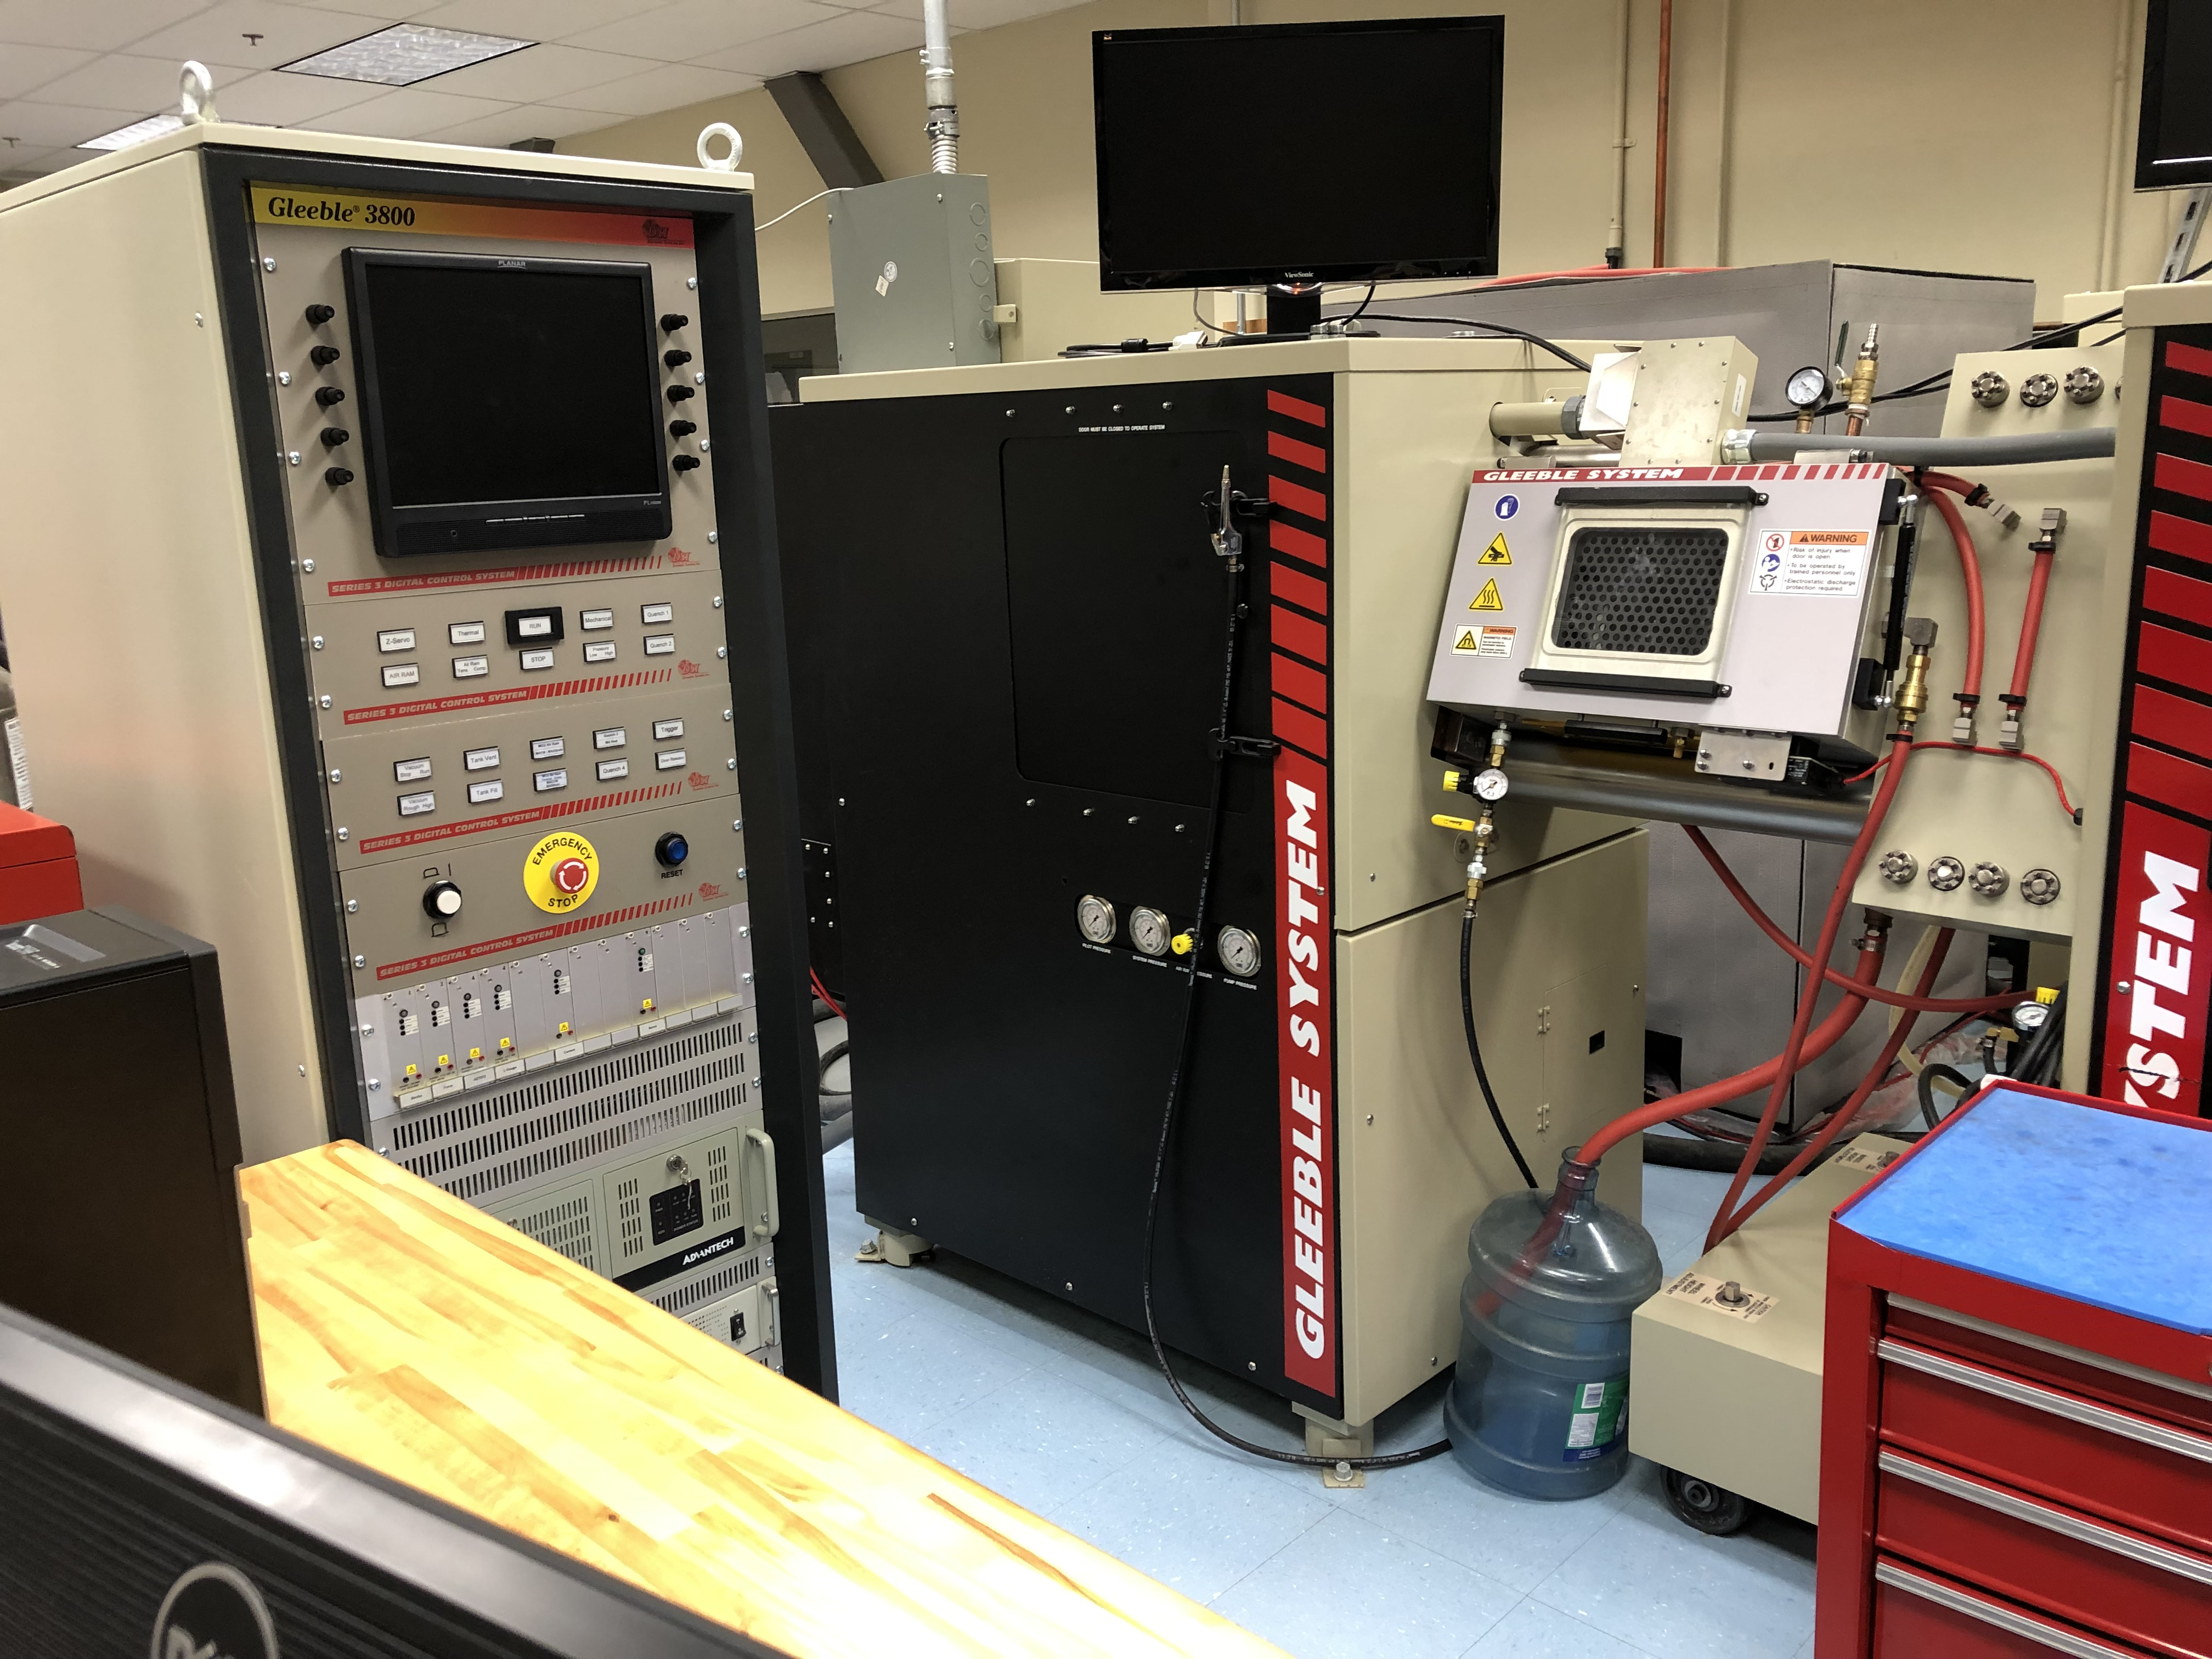
\includegraphics[width=0.7\columnwidth]{Figures/Gleeble-3800}
\caption{The Gleeble-3800 thermomechanical simulator system used for this study}
\label{fig:Gleeble3800}
\end{figure}

Thin tantalum sheets were used as a lubricating material at the contact surface of the anvils and samples to minimize friction during testing. As shown in Figure \ref{fig:GleebleProcess}, the samples were heated to a temperature of $1260$°C with a heating rate of $2$°C/s and held at this temperature for $5$~min to eliminate thermal gradients. They were then cooled with a rate of $1$°C/s to the test temperature and then held at constant temperature for $1$~min before deformation. During the compression phase, the temperature of the specimen is kept constant by the thermal control system of the machine. After compression, the specimen is quickly quenched to freeze its microstructure for later analysis. Figure \ref{fig:GleebleProcess} also shows the aspects of the specimens before and after the compression test: $h_0$ and $R_0$ are the height and radius before compression and $h$, $R_M$ and $R_T$ are the height, large radius and small radius of the specimen after compression, respectively.

\begin{figure}[!ht]
\centering
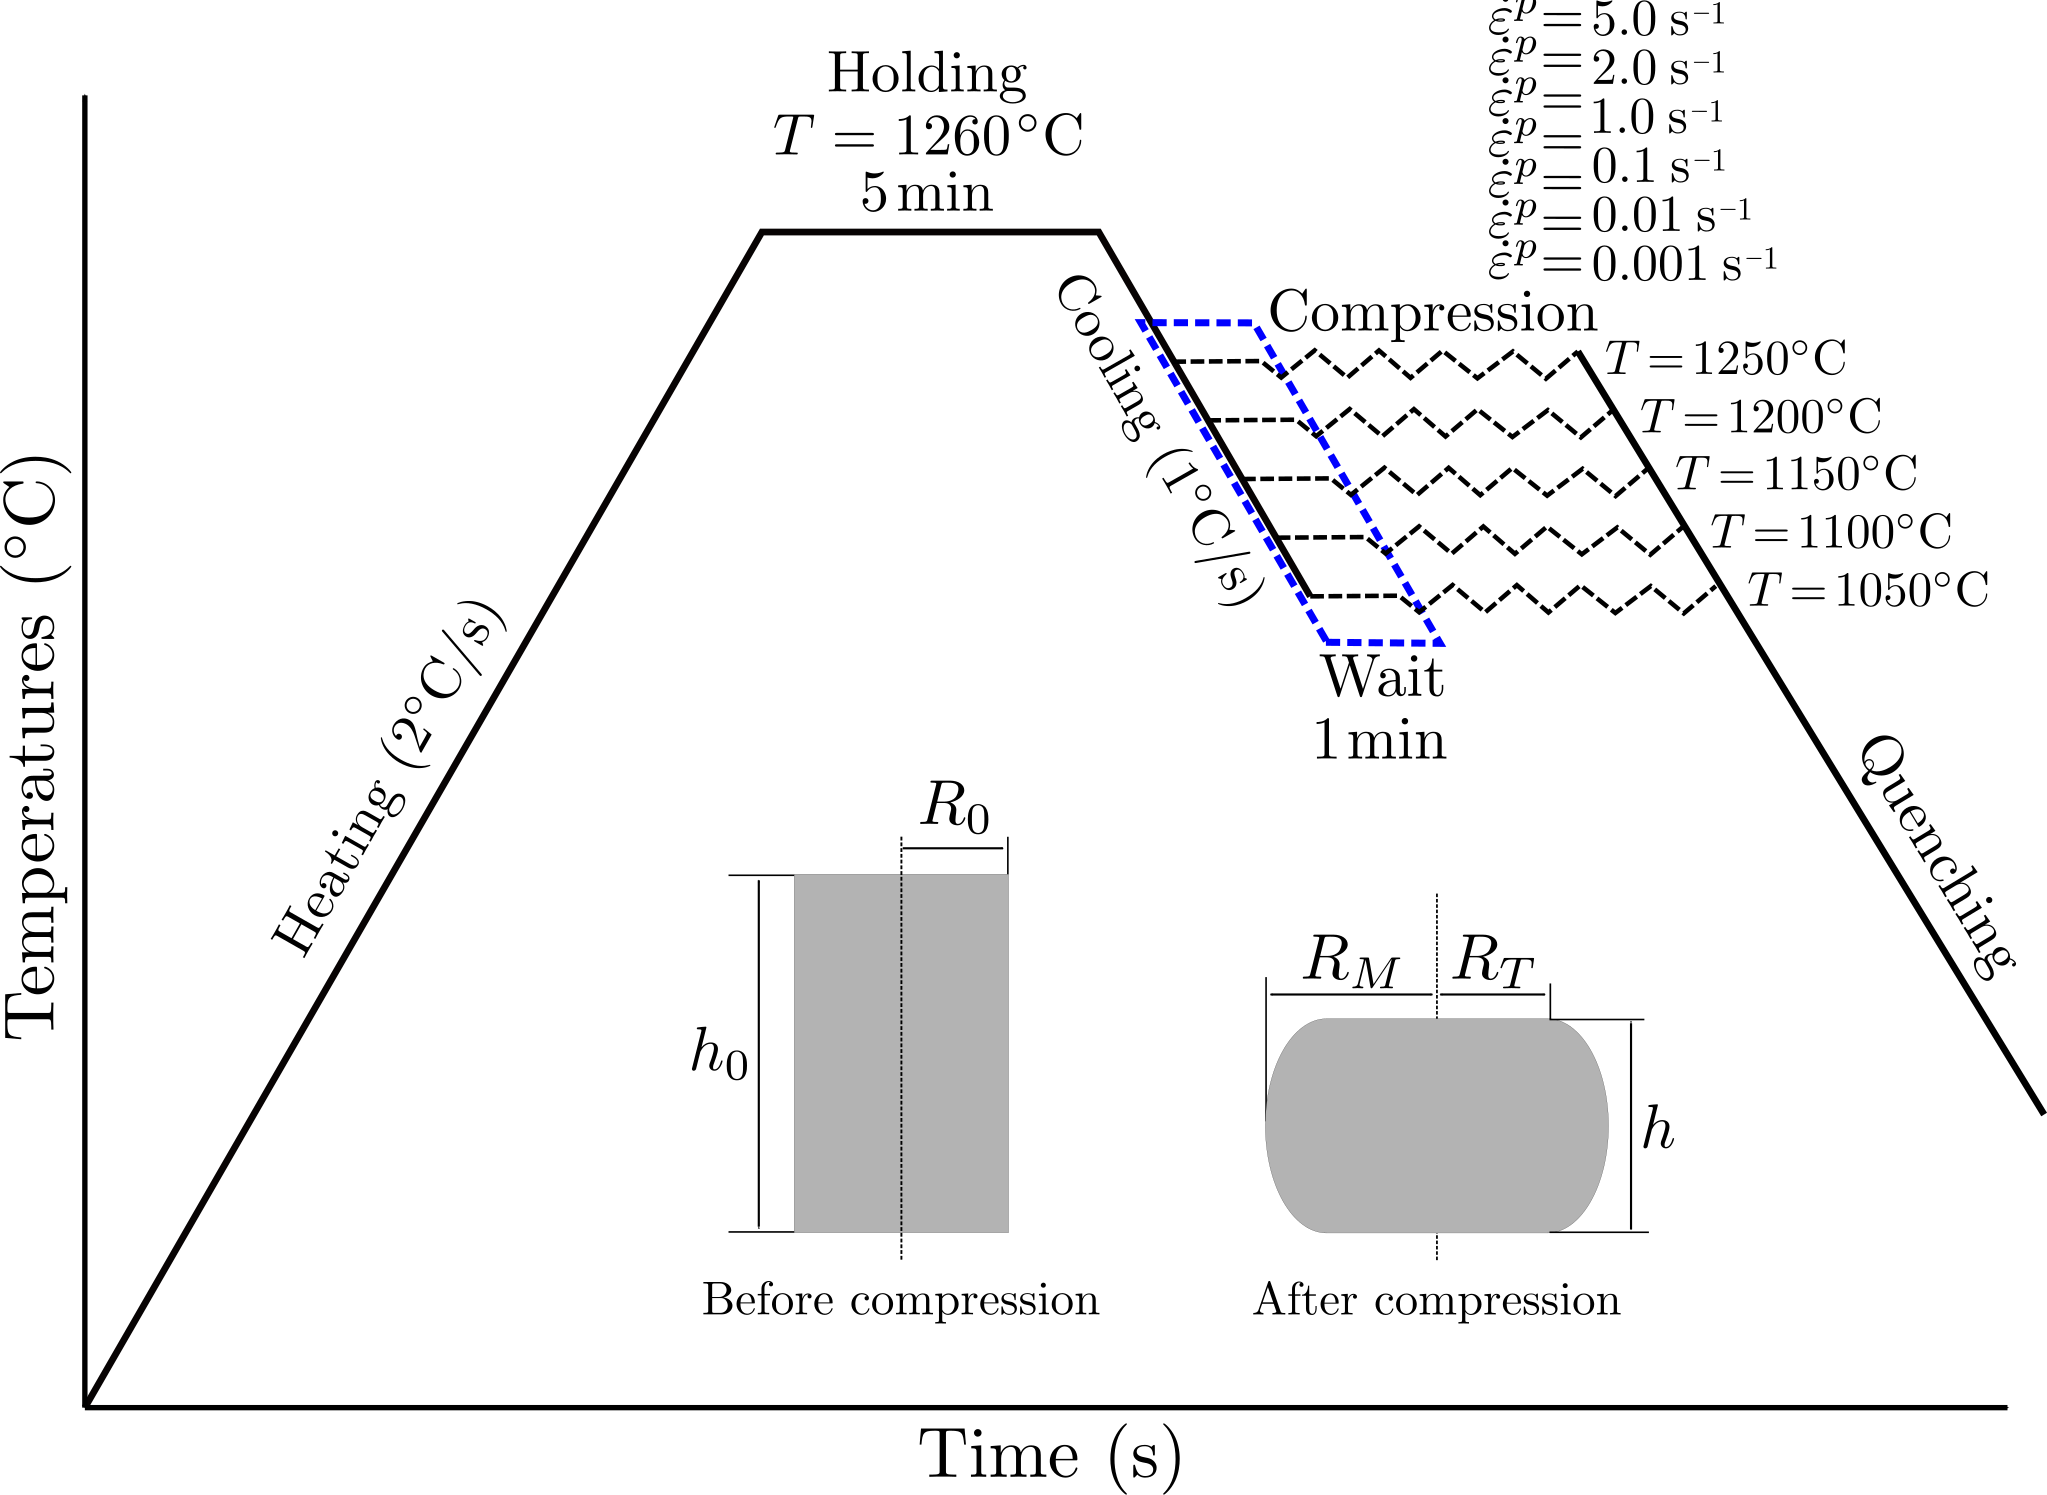
\includegraphics[width=0.8\columnwidth]{Figures/GleebleProcess}
\caption{Schematic diagram of the experimental process.}
\label{fig:GleebleProcess}
\end{figure}

%------------------------------------------------------------------------
\subsection{Compression tests results}
%------------------------------------------------------------------------

The set of flow stress $\sigma^y$ versus plastic strain $\varepsilon^p$ curves obtained from compression tests performed on the Gleeble-3800 simulator for each test condition ($6$ strain rates and $5$ temperatures) is presented in Figure \ref{fig:rawData}. The overall behavior of these curves shows that the flow stress $\sigma^y$ increases with increasing strain rate $\mdot\varepsilon^p$ but decreases with increasing temperature $T$. It should be noted that the plastic strain also influences the flow stress. Indeed, for the lowest strain rates $\mdot\varepsilon^p$, the flow stress $\sigma^y$ increases with the plastic strain $\varepsilon^p$ until a value of about $\varepsilon^p=0.2$ to $0.3$, then decreases to maintain a more or less constant value until the end of the test. For the highest strain rates ($1.0~\text{s}^{-1}$, $2.0~\text{s}^{-1}$, and $5.0~\text{s}^{-1}$), the flow stress increases throughout the test. One reason for the slight increase in stress at low strain rates when the strain is large is due to friction between the sample and the anvil during the test. For low strain rates, the effect of lubrication decreases over time and thus friction increases. This results in a progressive increase of the flow stress.

\begin{figure}[!ht]
\centering
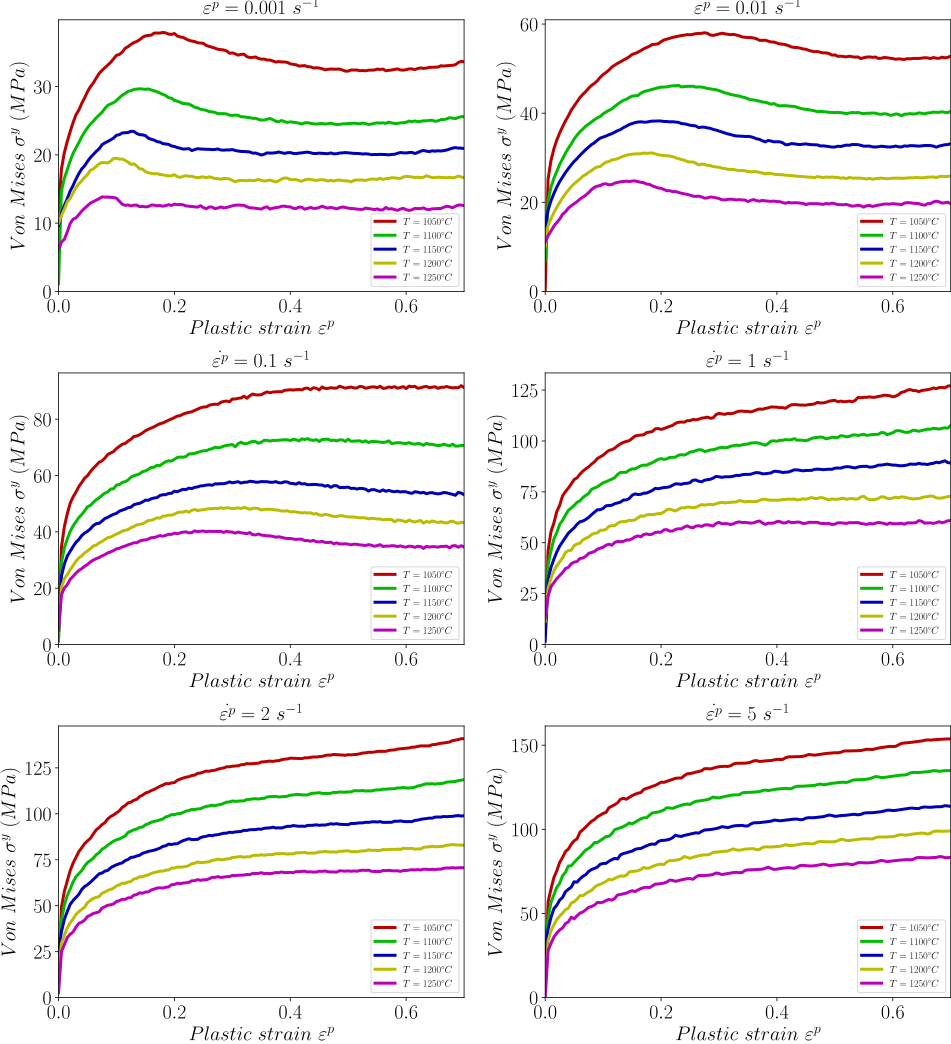
\includegraphics[width=1.02\columnwidth]
{Figures/rawData}
\caption{Flow stress-strain curves of AISI P20 alloy at various temperatures and strain rates.}
\label{fig:rawData}
\end{figure}

To explain the overall flow stress behavior observed in this test, we will rely on two fundamental phenomena that can be observed during a compression test: Dynamic Recovery (DRC) and Dynamic Recrystallization (DRX). At the beginning of the deformation of the sample in compression, the amount of dislocations increases and they begin to move within the material, which leads to a rapid increase in stress (strain hardening phenomenon). As the strain continues to increase, many dislocations are in motion, leading to a stress relaxation phenomenon, generally known as DRC. This DRC mechanism contributes to the decrease in the number of dislocations due to their combination with another dislocation or due to their integration into a grain boundary. Some of these dislocations reorganize and then form sub-grains within the initial grains of the material. The combination of these dislocations moderates the increase in the number of dislocations related to work hardening and thus controls the amount of strain energy stored in the material, which influences the increase in flow stress. The dynamic recrystallization concerns the germination of new grains, at the borders or inside the initial grains. These two phenomena explain the different shapes of the flow stress curves observed for this alloy. As an example, Figure \ref{fig:Micrography} show the microstructures of AISI P20 held during $5$~min at $1260$°C before and after the compression phase. As observed on the flow curves, it can be seen by comparing these two micrographs that recrystallization is almost complete for this temperature and strain rate within the sample \OP{What are the temperature and strain rate related with this micrography}. From the results reported in Figure \ref{fig:rawData}, the identification of the parameters of the six flow laws proposed in this work will be presented in the next section in order to predict the behavior of the material in any test condition.

\begin{figure}[!ht]
\centering
\begin{subfigure}[b]{0.45\textwidth}
\centering
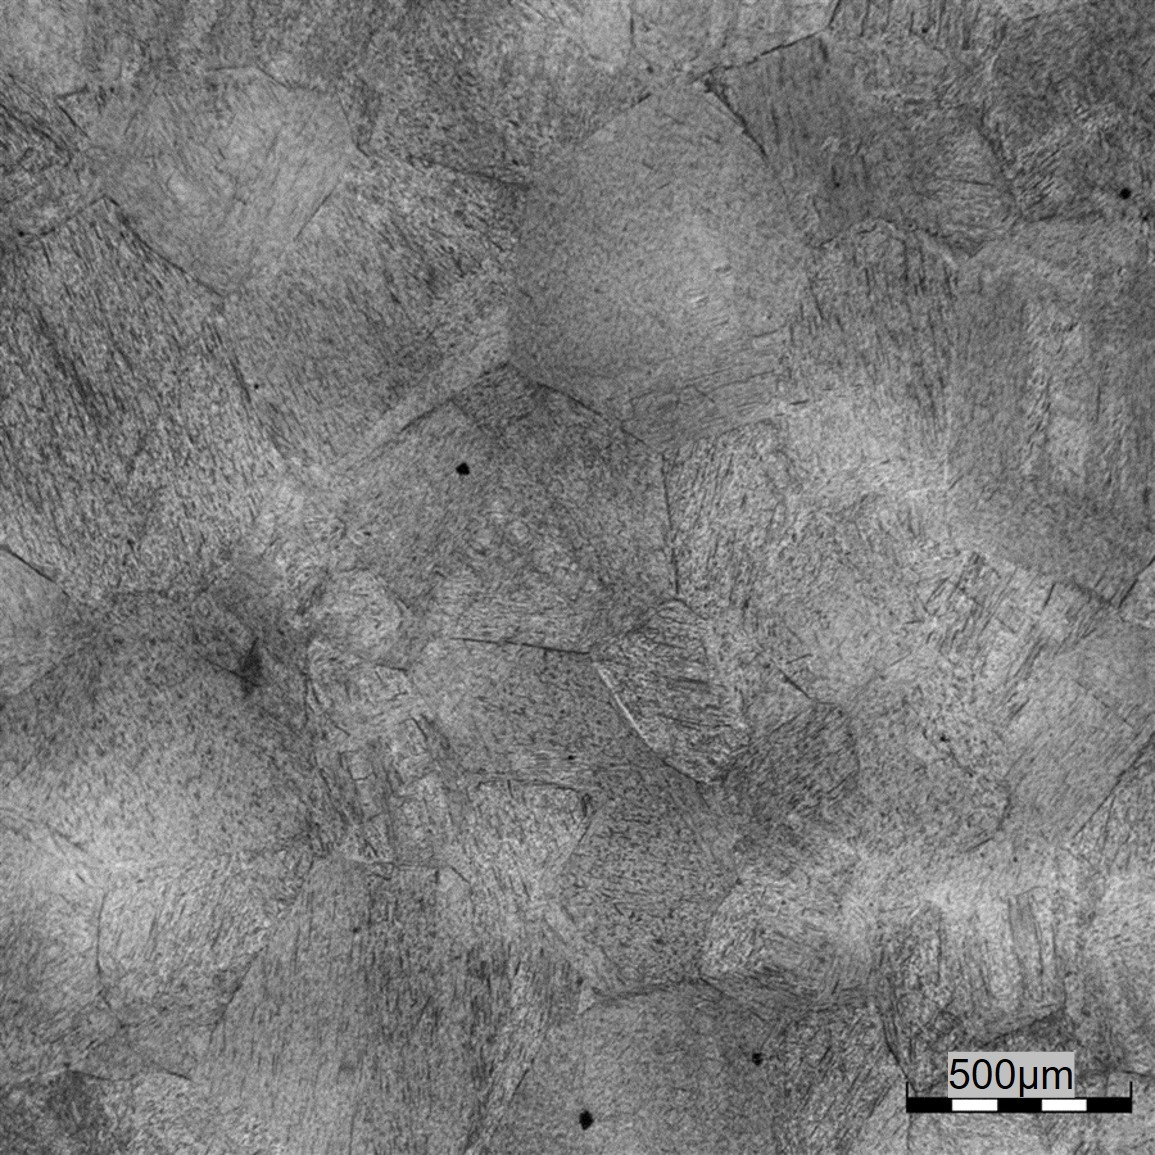
\includegraphics[width=\textwidth]{Figures/BeforeCompM}
\caption{Before hot compression}
\end{subfigure}
\hfill
\begin{subfigure}[b]{0.45\textwidth}
\centering
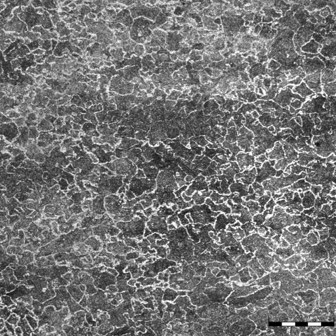
\includegraphics[width=\textwidth]{Figures/AfterCompM}
\caption{After hot compression}
\end{subfigure}
\caption{Optical micrographs of the AISI P20 steel before and after hot compression.}
\label{fig:Micrography}
\end{figure}

%-------------------------------------------------------------------------
\section{Phenomenological constitutive flow laws\label{sec:ConstLaws}}
%-------------------------------------------------------------------------
The complete characterization of the thermomechanical behavior of a material is very important before its use in numerical simulations. This characterization usually involves experimental tests that serve as a basis for the development of constitutive laws. As mentioned in the introduction, many constitutive laws exist today, and selecting one of them based on explicit criteria hinders the development of computational models for new materials. Since the purpose of this work is to compare ANN model to analytical models it is important to justify the choice of the analytical models presented here among the many that exist in the literature. Among the most widely used analytical models nowadays, the Johnson-Cook (JC) model is the most used due to its simplicity of use linked to the number of its reduced and easy to obtain parameters. It should be noted that it is not the best model but the most integrated in finite element software. Hence the existence of several modified forms of this model. The Zerilli-Armstrong model, and particularly its modified form (MZA), is also widely known since it tries to provide solutions to the shortcomings of the JC model, particularly with regard to the coupling of physical parameters. Hence its use also in this study. In this perspective, the Hansel Spittel model (HS)is also one of the most widely used models in numerical simulation of casting and forging operations as it is integrated in the FORGE software. Also, the method of identifying its parameters is very simple to do as it is done in one step. Of course, it has its limitations as will be shown in the following sections. Furthermore, the Arrhenius model will be used in this study because it is one of the models that not only provides a good prediction of the flow stress but also takes into account the physical parameter Q (the deformation activation energy coefficient) which is of great importance in the study related to the microstructural analysis of materials. The PTM model is also used in this study as it is a model whose formulation does not impose a number of parameters a priori and has proven its ability in our previous work and therefore we want to test it on this type of material as it is formulated to fit any material.
%-------------------------------------------------------------------------
\subsection{Johnson--Cook model\label{sec:JC}}
%-------------------------------------------------------------------------
The JC model as mentioned above, is one of the most widely used analytical models as it can be applied to several materials under different conditions of strain, strain rate and temperature. However, the formulation of this model does not take into account the simultaneous effect of strain, strain rate and temperature. Indeed, it is formulated by describing the effect of each physical parameter (strain, strain rate and temperature) separately as a factor in the mathematical expression of the model. Hence its inability to describe the phenomenon of temperature-induced softening. The equation that describes this model is given as follows \cite{Johnson-1985}:
\begin{equation}
\label{eq: JCmodel}
\sigma^y = \left(A + B\varepsilon^{p^n}\right)\left(1+C\ln\mdot\varepsilon^*\right)\left(1-T^{*^m}\right)
\end{equation}
Where $\sigma^y$ is the equivalent stress flow stress, $\varepsilon^p$ is the plastic strain, ($A=\sigma^y_0$) is the elastic limit of the material, $B$ is the strain hardening's coefficient, $n$ is the strain hardening's exponent. $C$ and $m$ are the material constants that describe the strain rate hardening and thermal softening exponent respectively. $\mdot\varepsilon^*$ is the dimensionless strain rate which is given by $\mdot\varepsilon^* = \mdot\varepsilon^p/\mdot\varepsilon_0$. $\mdot\varepsilon^p$ and $\mdot\varepsilon_0$ are strain rate and reference strain rate respectively. $T^{*^m} = (T-T_0)/(T_m - T_0)$ is homologous temperature where $T, T_m$ and $T_0$ are the déformation temperature, meltinng temperature ($1460$°C in our case) and reference temperature respectively. For the determination of the parameters of the analytical models, the reference values for strain rate and temperature are $2.0$ and $1050$°C respectively and the value of $A$ is $43.0988$ MPa. Here after datailed the steps for determination of the JC model parameters.
At the reference strain rate, Equation \ref{eq: JCmodel} becomes:
\begin{equation}
\label{eq: JCbn}
\sigma^y = A + B\varepsilon^{p^n}
\end{equation}
Taking the natural logarithm on both sides of Equation \ref{eq: JCbn} we have:
\begin{equation}
\label{eq:JClog1}
\ln\left(\sigma^y-A\right)= \ln(B) + n\ln\varepsilon^p
\end{equation}
By plotting $\ln(\sigma^y-A)$ \versus $\ln\varepsilon^p$ (Figure \ref{fig:JCSigmaAB}) from Equation \ref{eq:JClog1}, $n$ and $B$ can be obtained as slope and intercept respectively. Thus, for a strain value equal to $0.1$ the values of these two parameters are $n=0.313969$ and $B=114.518$.
\begin{figure}[!ht]
\centering
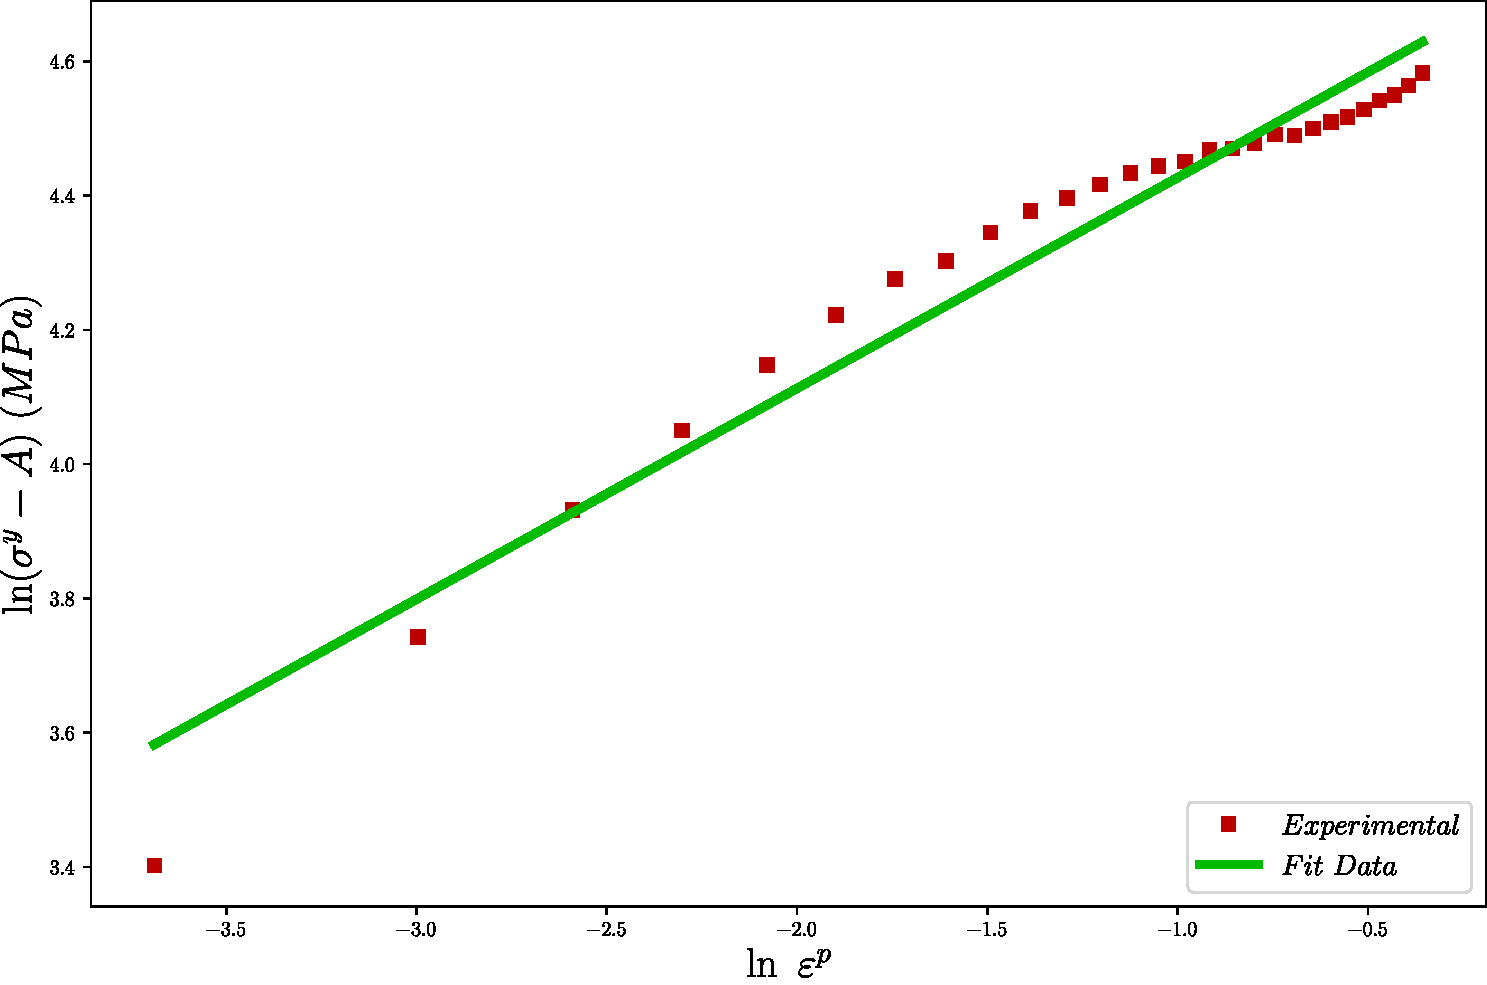
\includegraphics[width=0.9\columnwidth]
{Figures/JCSigmaAB}
\caption{Relationship between $ln(\sigma^y -A)$ and $\ln(\varepsilon^p)$ at $1050$°C and $0.1$}
\label{fig:JCSigmaAB}
\end{figure}
\FloatBarrier
Once the parameters $A$, $B$ and $n$ are known and at the reference temperature, the Equation \ref{eq: JCmodel} becomes:
\begin{equation}
\frac{\sigma^y}{A + B\varepsilon^{p^n}} = 1 + C\ln\mdot\varepsilon^*
\end{equation}
From this equation one can easily obtain the parameter $C$ using the linear fitting method for each strain value and averaging all these values as shown in Figure \ref{fig:JCSigmaAB1} the value is $0.0995438$.
\begin{figure}[!ht]
\centering
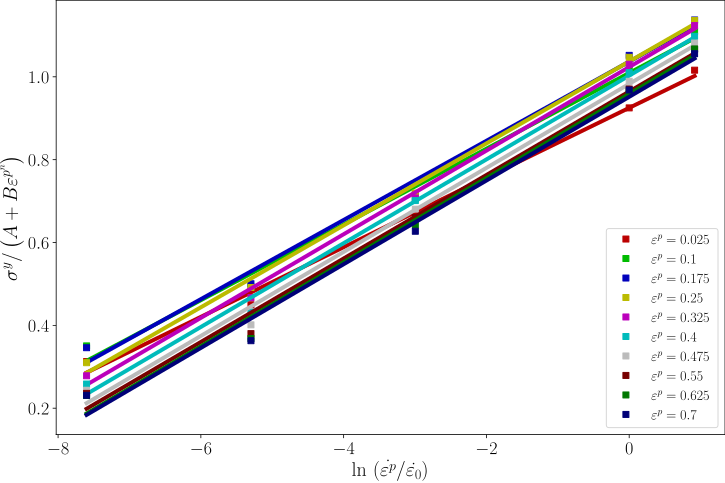
\includegraphics[width=0.9\columnwidth]
{Figures/JCSigmaAB1}
\caption{Relationship between $\sigma^y/(A+ B\varepsilon^{p^n})$ and $\ln(\dot{\varepsilon}^*)$}
\label{fig:JCSigmaAB1}
\end{figure}
The $m$ parameter is determined at the reference strain rate. Under this condition, the Equation \ref{eq: JCmodel} can be written as following:
\begin{equation}
\frac{\sigma^y}{A + B\varepsilon^{p^n}} = 1 - T^{*^m}
\end{equation}
Taking the natural logarithm of both sides of that equation, we have:
\begin{equation}
\ln\left(1 - \frac{\sigma^y}{A + B\varepsilon^{p^n}}\right)  = m\ln T^*
\end{equation}
Plotting $\ln\left(1 - \frac{\sigma^y}{A + B\varepsilon^{p^n}}\right)$ as a function of $\ln T^*$ allows us to get the parameter $m$ as a slope for all values of the deformation by averaging them and the value is $0.898932$. Figure \ref{fig:JCSigmaT} illustrates this determination for some deformations.
\begin{figure}[!ht]
\centering
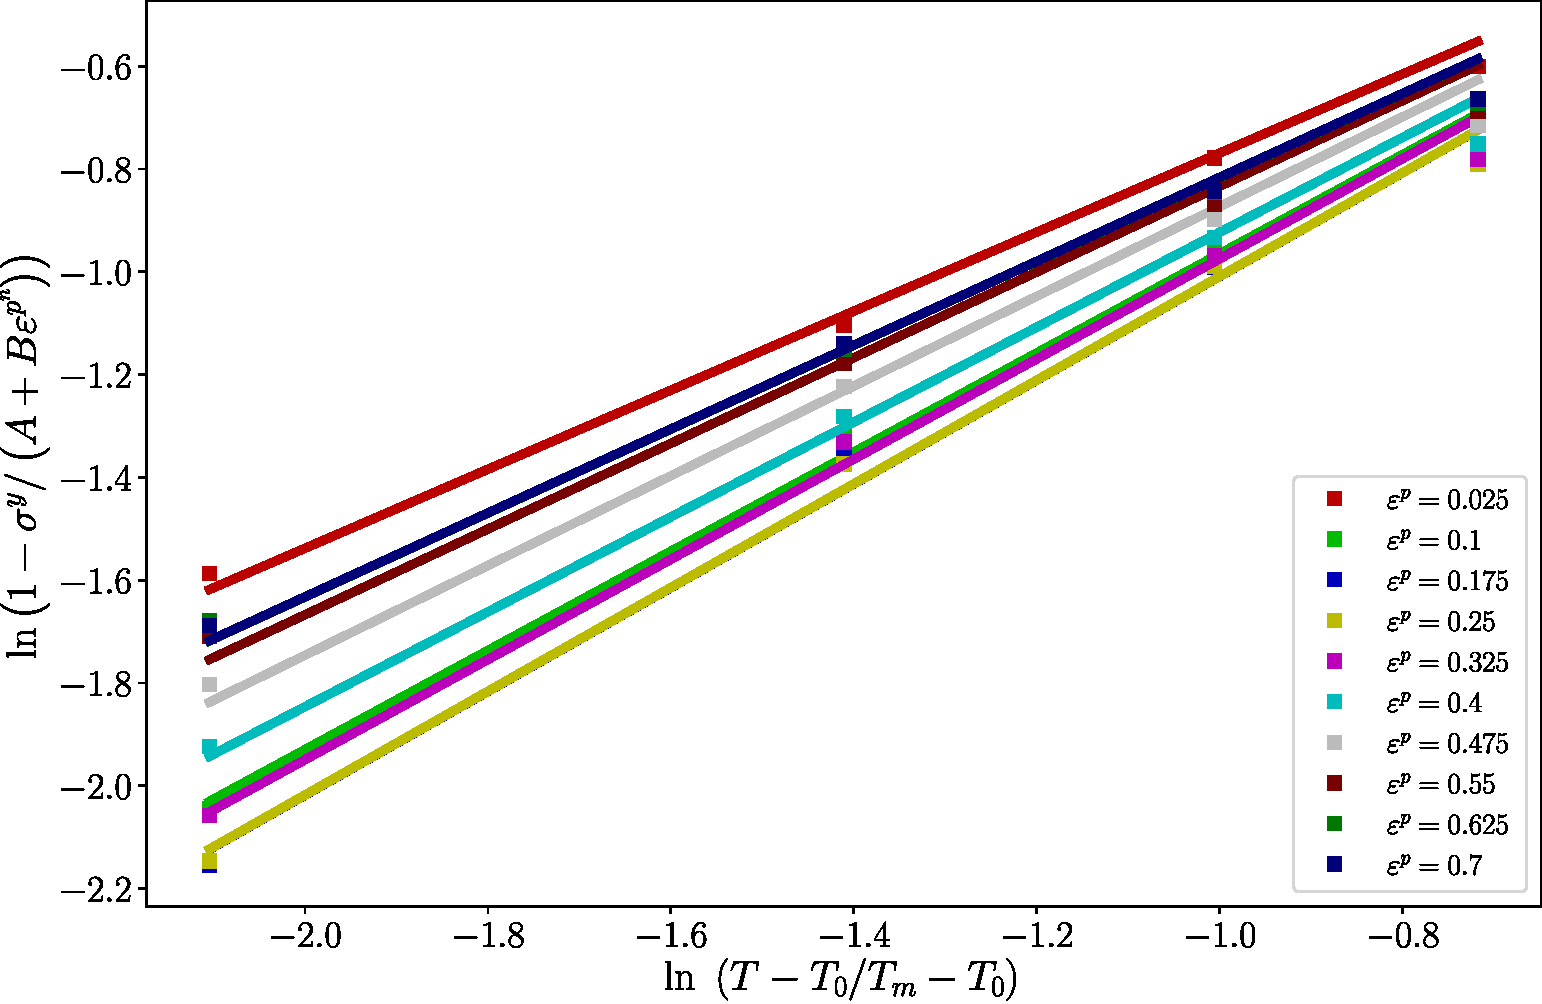
\includegraphics[width=0.85\columnwidth]
{Figures/JCSigmaT}
\caption{Relationship between $\ln\left(1 - \sigma^y/\left(A + B\varepsilon^{p^n}\right)\right)$ and $\ln T^*$}
\label{fig:JCSigmaT}
\end{figure}

The predicted and experimental values are compared, as shown in Figure \ref{fig:iCorrelationJC}. The JC model is not much suitable to describe the flow behavior of AISI P20 within entire deformation condition, and predicted values show a monotonous downward trend at various strain rates. The deviation between predicted values and experimental values is large for the low strain rates and almost acceptable at high strain rates. All parameters of JC model are in Table \ref{tab: JCparameters}.
\begin{figure}[!ht]
\centering
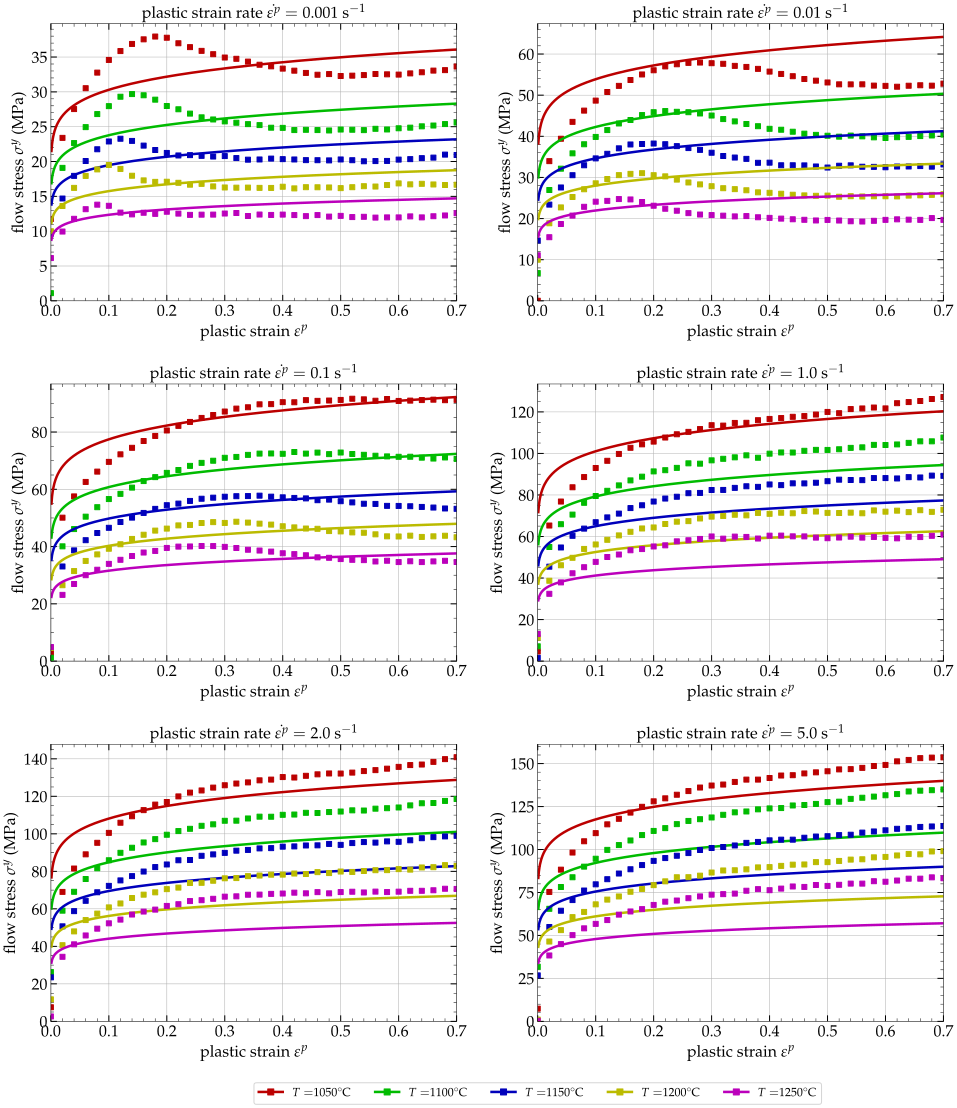
\includegraphics[width=1.02\columnwidth]
{Figures/CompExpJC}
\caption{Comparison between the experimental and predicted flow stresses by JC model}
\label{fig:iCorrelationJC}
\end{figure}
\begin{table}[h!]
\centering{}
\caption{Parameters' constants of Johnson-Cook Model}
\begin{tabular}{lccccc}
\hline
&         &             &		   &		  &\\
Parameters&$A(\text{MPa})$    &$B(\text{MPa})$        & $n$     & $C$   & $m$       \\
&         &             &		   &	     &	    \\
\hline
Values&$43.0988$&$114.518$& $0.313969$&$0.0995438$&$0.898932$\\
\hline
\label{tab: JCparameters}
\end{tabular}
\end{table}
%-------------------------------------------------------------------------
\subsection{Modified Zerilli-Armstrong model\label{sec:MZA}}
%-------------------------------------------------------------------------

As mentioned earlier, Johnson-Cook's law, widely used in the scientific community and implemented as a base in the Abaqus FEM code, is an empirical model for which the effects of strain, strain rate, and temperature on material behavior are considered separately. Since a coupling exists in reality between these three variables, it is preferable to opt for a Zerilli-Armstrong (ZA) model \cite{Hull-2011}. But the original for of ZA model has some limitations due to the fact that it is considered as two terms and to ameliorate that formulation Samantaray \eal \cite{Samantaray-2009} proposed a modified form given by the following equation:
\begin{equation}
\label{eq:MZA-model}
\sigma^y = \left(C_{1}+C_{2}\varepsilon^{p^n}\right) \exp\left[-\left(C_{3}+C_{4}\varepsilon^p\right)\left(T-T_0\right) + \left(C_{5}+C_{6}\left(T-T_0\right)\right)\ln\left( \frac{\mdot\varepsilon^p}{\mdot{\varepsilon}_0}\right)\right]
\end{equation}
where the $7$ coefficients $C_i$ and $n$ are the parameters of the model to be identified for a given material. The formulation of the model can be found in \cite{Samantaray-2009} and determination of its parameters is sumarized as following.

Considering the expression of the model given by Equation (\ref{eq:MZA-model}), parameter $C_1$ is deduced direcly from $\sigma^y(\varepsilon^p=0,T=T_0,\mdot\varepsilon^p=\mdot{\varepsilon}_0)$. When the current strain rate $\mdot\varepsilon^p$ is identical to the reference strain rate $\mdot{\varepsilon}_0$, the Equation (\ref{eq:MZA-model}) becomes :
\begin{equation}
\sigma^y = \left(C_{1}+C_{2}\varepsilon^{p^n}\right) \exp\left[-\left(C_{3}+C_{4}\varepsilon^p\right)\left(T-T_0\right)\right]
\end{equation}
Taking the logarithm of the previous relationship we have :
\begin{equation}
\ln\sigma^y = \ln\left(C_{1}+C_{2}\varepsilon^{p^n}\right)-\left(C_{3}+C_{4}\varepsilon^p\right)\left(T-T_0\right)
\end{equation}
By plotting the function $\ln\sigma^y\left(T-T_0\right)$ the y-intercept and the slope of this line can be deduced as $I_1=\ln\left(C_1+C_2\varepsilon^{p^n}\right)$ and $S_1=-\left(C_3+C_4\varepsilon^p\right)$.
From the expression of $I_1$ we can write:
\begin{equation}
\ln\left(\exp(I_1)-C_1\right) = \ln C_2+n\ln\varepsilon^p
\end{equation}
By plotting the function $\ln\left(\exp(I_1)-C_1\right)$ versus $\ln\varepsilon^p$ we can deduce $n$ and $C_2$. The plot of $S_1$ versus $\varepsilon^p$ allows deducing $C_3$ and $C_4$ from the y-intercept and the slope, respectively. Once the first four terms of the model are calculated, we can now take the logarithm of the entire MZA model given by Equation (\ref{eq:MZA-model}).
\begin{equation}
\ln\sigma^y = \ln\left(C_{1}+C_{2}\varepsilon^{p^n}\right) - \left(C_{3}+C_{4}\varepsilon^p\right)\left(T-T_0\right) + S_2\ln\left( \frac{\mdot\varepsilon^p}{\mdot{\varepsilon}_0}\right)
\end{equation}
with $S_2=C_5+C_6\left(T-T_0\right)$. Finally, the graph $\ln\sigma^y$ versus $ \ln(\mdot\varepsilon^p/\mdot{\varepsilon}_0)$ allows deducing $C_5$ and $C_6$ from the slope $S_2$. The parameters of MZA model are given in the Table \ref{tab: MZAparameters} while its prediction are shown in Figure \ref{fig:iCorrelationMZA}. It can be seen from those figures that the MZA model as JC model is not suitable to describe experimental at low strain rates but much better for high strain rates. The deviation between the predicted values and the experimental values is large because this model has problem to correctly describe the softening in its formulation. That is aspect of the limitations of that model as presented in \cite{TizeMha-2022}.
\begin{table}[h!]
\centering{}
\caption{Parameters' constants of Modified-Zerilli-Armstrong Model}
\begin{tabular}{lllllllc}
\hline
&         &             &		   &		 &			   &&\\
Parameters&$C_1(\text{MPa})$    &$C_2(\text{MPa})$        & $C_3(\times10^{-5})$     & $C_4(\times10^{-5})$   & $C_5(\times10^{-5})$       &$C_6(\times10^{-5})$&$n$\\
&         &             &		   &	     &	           &&\\
\hline
Values&$43.0988$&$112.975$& $330.976$&$4.27581$&$14106.3$&$17.4178$&$0.305028$\\
\hline
\label{tab: MZAparameters}
\end{tabular}
\end{table}
\begin{figure}[!ht]
\centering
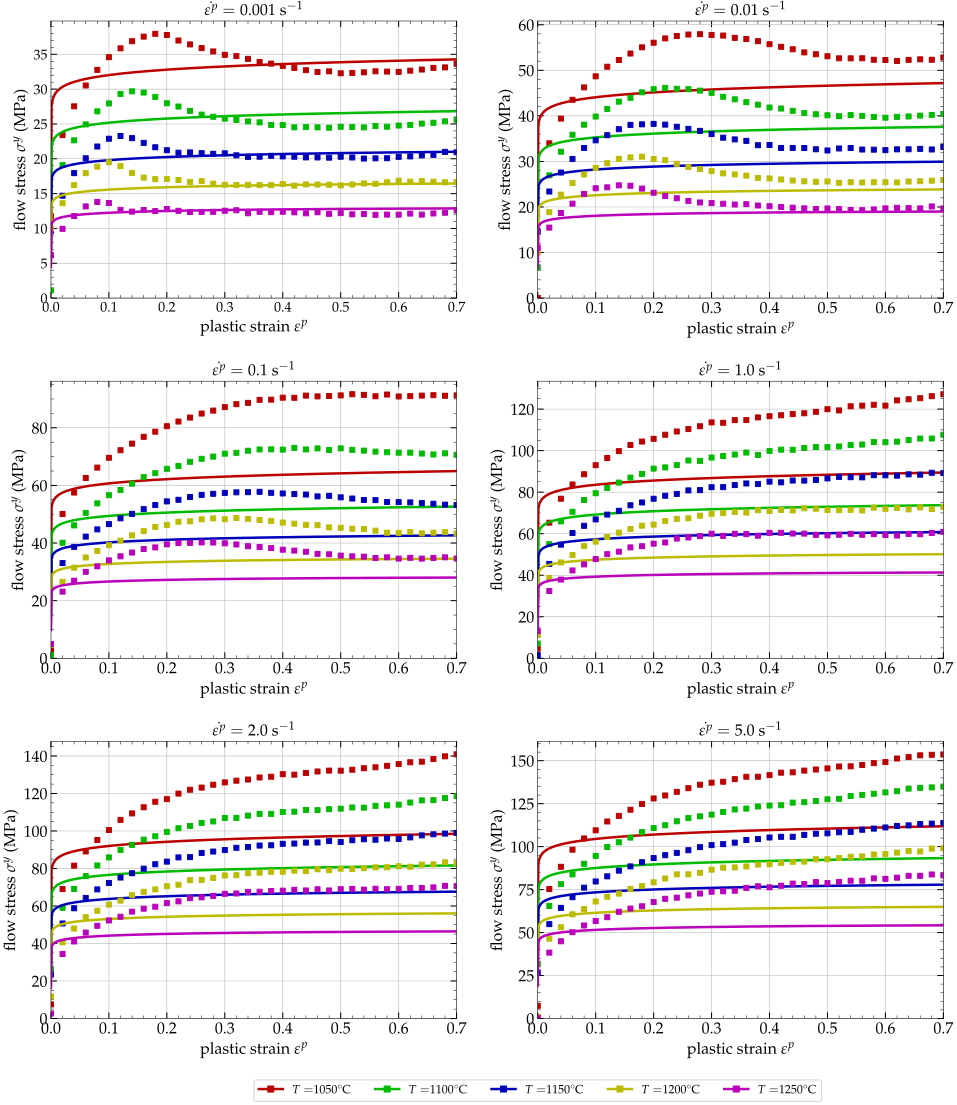
\includegraphics[width=1.02\columnwidth]
{Figures/CompExpMZA}
\caption{Comparison between the experimental and predicted flow stresses by MZA model}
\label{fig:iCorrelationMZA}
\end{figure}
\FloatBarrier

%-------------------------------------------------------------------------
\subsection{Hansel and Spittel\label{sec:HSmodel}}
%-------------------------------------------------------------------------
The Hansel-Spittel model is one of the least known models in terms of its  integration in software for finite element simulation although the determination of its parameters is easier than the JC model. A single programming command is sufficient for its identification. However, this model has some difficulties as it loses its accuracy when all parameters are taken into account. For this reason, several authors limit its use to $5$ or $6$ parameters \cite{Chadha-2018, Rudnytskyj-2020, Mehtedi-2015}. In this paper the good predictions are with $5$ parameters summarized in Table \ref{tab: HSparameters}. The equation of the model is given by the following relation:
\begin{figure}[!ht]
\centering
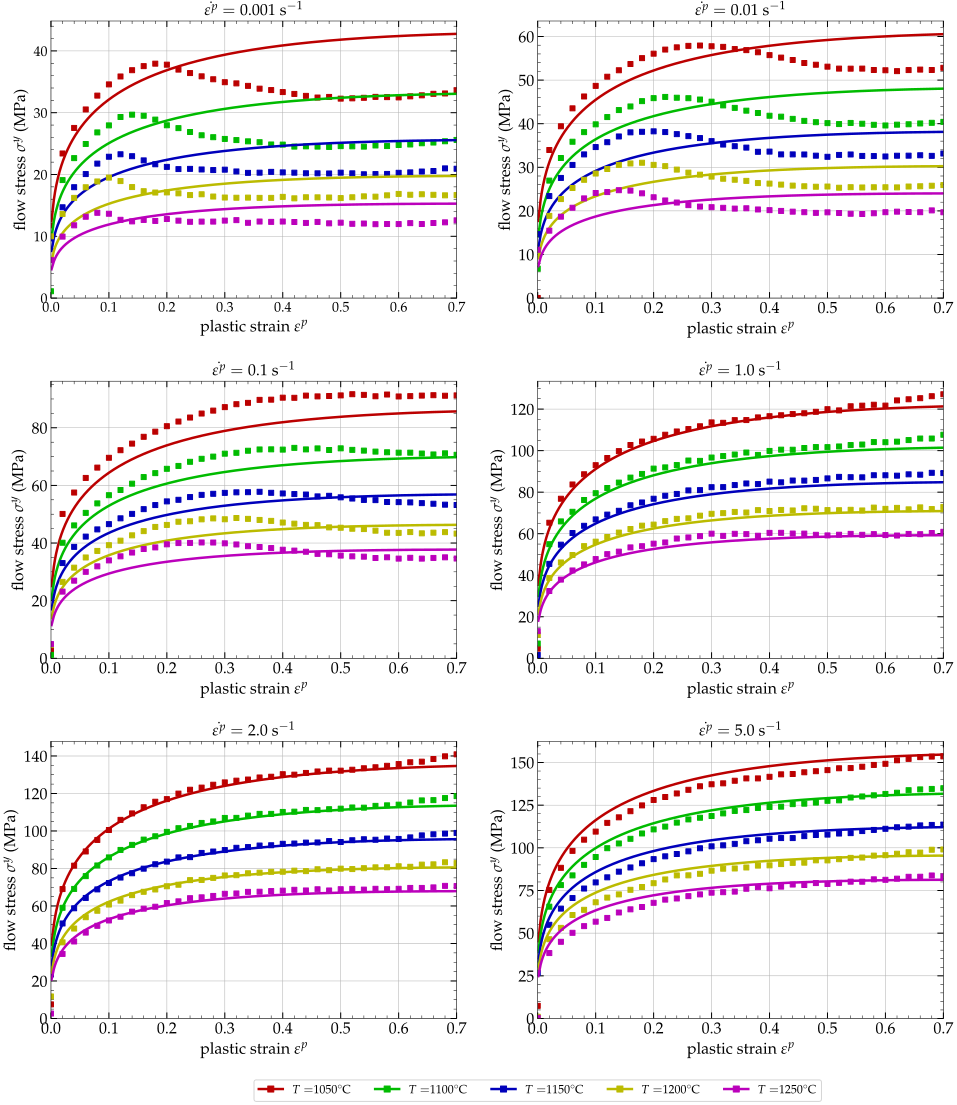
\includegraphics[width=1.02\columnwidth]
{Figures/CompExpHS}
\caption{Comparison between the experimental and predicted flow stresses by HS model}
\label{fig:iCorrelationHS}
\end{figure}
\begin{equation}
\sigma^y = Ae^{m_1T}\varepsilon^{p^{m_2}}\mdot\varepsilon^{p^{m_3}}e^{\frac{m_4}\varepsilon^p}(1+\varepsilon^p)^{m_5T}e^{m_6\varepsilon^p}\mdot\varepsilon^{p^{m_7T}}T^{m_8}
\end{equation}
Where $\sigma^y$ is the flow stess, $\varepsilon^p$ strain, $\mdot\varepsilon^p$ strain rate and $T$ temperature. The other coefficients $A$ and $m_j$ are model constants up to $m_5$ for our case. Comparison of predicted values of the HS model and experimental values is shown in Figure \ref{fig:iCorrelationHS}. It appears that this model as well as the previous ones do not predict the experimental well and the gap is relatively large. This shows that this model is not appropriate for the characterisation of this alloy.
\begin{table}[h!]
\centering{}
\caption{Parameters' constants of Hansel and Spittel Model}
\begin{tabular}{llccccc}
\hline
&         &             &		   &		 &			   &\\
Parameters&$A_0(\text{MPa})$    &$m_1$        & $m_2$     & $m_3$   & $m_4$       &$m_5$\\
&         &             &		   &	     &	           &\\
\hline
Values&$9254.77$&$-0.00375057$& $0.208975$&$0.184238$&$-0.00287837$&$-0.000583287$\\
\hline
\label{tab: HSparameters}
\end{tabular}
\end{table}
%----------------------------------------------------------------------------------
\subsection{Arrhenius model (AR model), \label{sec:ARmodel}}
%----------------------------------------------------------------------------------
The Arrhenius tye model is one of the most widely used models, especially when it comes to studying the microstructure of the material. Indeed, this model takes into account the physical phenomena that describe the behavior of the material and also the relations between stress ($\sigma^y$), strain ($\varepsilon^p$), the strain rate ($\mdot\varepsilon^p$) and the temperature ($T$) could be expressed in form of the power law, the exponential law and the hyperbolic sine type equation. This facilitates an easier description of the phenomenon of softening observed in material due to the increase in temperature. The following equations describe the Arrhenius model.
\begin{equation}
\label{eq:ARmodel1}
\mdot\varepsilon^p = A_1\sigma^{y^{n_1}}\exp\left(-\frac{Q}{RT}\right) \qquad (for ~~\alpha\sigma^y < 0.8)
\end{equation}
\begin{equation}
\label{eq:ARmodel2}
\mdot\varepsilon^p = A_2\exp(\beta\sigma^y)\exp\left(-\frac{Q}{RT}\right) \qquad (for ~~\alpha\sigma^y > 1.2)
\end{equation}
\begin{equation}
\label{eq:ARmodel}
\mdot\varepsilon^p = A_3\left[\sinh(\alpha\sigma^y)\right]^{n_2}\exp\left(-\frac{Q}{RT}\right) \qquad (for ~~all\ \sigma^y)
\end{equation}
Where $\mdot\varepsilon^p$ is the strain rate ($s^{-1}$), $Q$ is the deformation activation energy ($KJmol^{-1}$), $R$ is the universal gas constant ($8.314\ J mol^{-1} K^{-1}$), $T$ is the absolute temperature ($K$) and $A_1, A_2, A_3, n_1$, $n_2, \beta$ and $\alpha(\beta/n_1)$ are the material constants. To take into account the effects of temperature and strain rate on the deformation, a parameter ($Z$) called Zener-Hollomon parameter is introduced whose expression is given as follows:
\begin{equation}
\label{eq:Zparam}
Z = \mdot\varepsilon^p\exp\left(\frac{Q}{RT}\right)
\end{equation}
By replacing the Equation (\ref{eq:ARmodel}) inton Equation (\ref{eq:Zparam}) it comes:
\begin{equation}
\label{eq:Zparam1}
Z = A_3\left[\sinh(\alpha\sigma^y)\right]^{n_2} \qquad \Rightarrow \qquad \sinh(\alpha\sigma^y) = \left(\frac{Z}{A_3}\right)^{1/n_2}
\end{equation}
Furthermore, it is known that:
\begin{equation}
arc\sinh(x) = \ln\left(x + \sqrt{1+x^2}\right)
\end{equation}
Therefore Equation (\ref{eq:Zparam1}) becomes and which is actually the Arhenius model:
\begin{equation}
\sigma^y = \frac{1}{\alpha}\ln\left\{\left(\frac{Z}{A_3}\right)^{1/n_2} + \left[1 + \left(\frac{Z}{A_3}\right)^{2/n_2}\right]^{1/2}\right\}
\end{equation}
To obtain the constitutive equation, all parameters $\alpha$, $Q$, $n_2$, and $A_3$ needed to be determined. The following part shows the calculation procedures of these material constants at $\varepsilon^p = 0.1$ as example. Taking the natural logarithm of Equations (\ref{eq:ARmodel1}) and (\ref{eq:ARmodel2}), the following relationships can be obtained:
\begin{equation}
\ln \sigma^y = \frac{1}{n_1}\ln \mdot\varepsilon^p -\frac{1}{n_1}\ln A_1 +  \frac{1}{n_1}\frac{Q}{RT}
\end{equation}
\begin{equation}
\sigma^y = \frac{1}{\beta}\ln \mdot\varepsilon^p - \frac{1}{\beta}\ln A_2 + \frac{1}{\beta}\frac{Q}{RT}
\end{equation}
From these two equations, we can easily deduce the parameters $n_1$ and $\beta$ as the slopes of the functions $\ln\sigma^y = f(\ln\mdot\varepsilon^p)$  and $\sigma^y = f(\ln\mdot\varepsilon^p)$ as shown in Figure \ref{fig:LnAlp} and Figure \ref{fig:LnSinhE0} for $\varepsilon^p = 0.1$. It should be noted that later in this document all values of strain will be taken into account.
\begin{figure}[!ht]
\centering
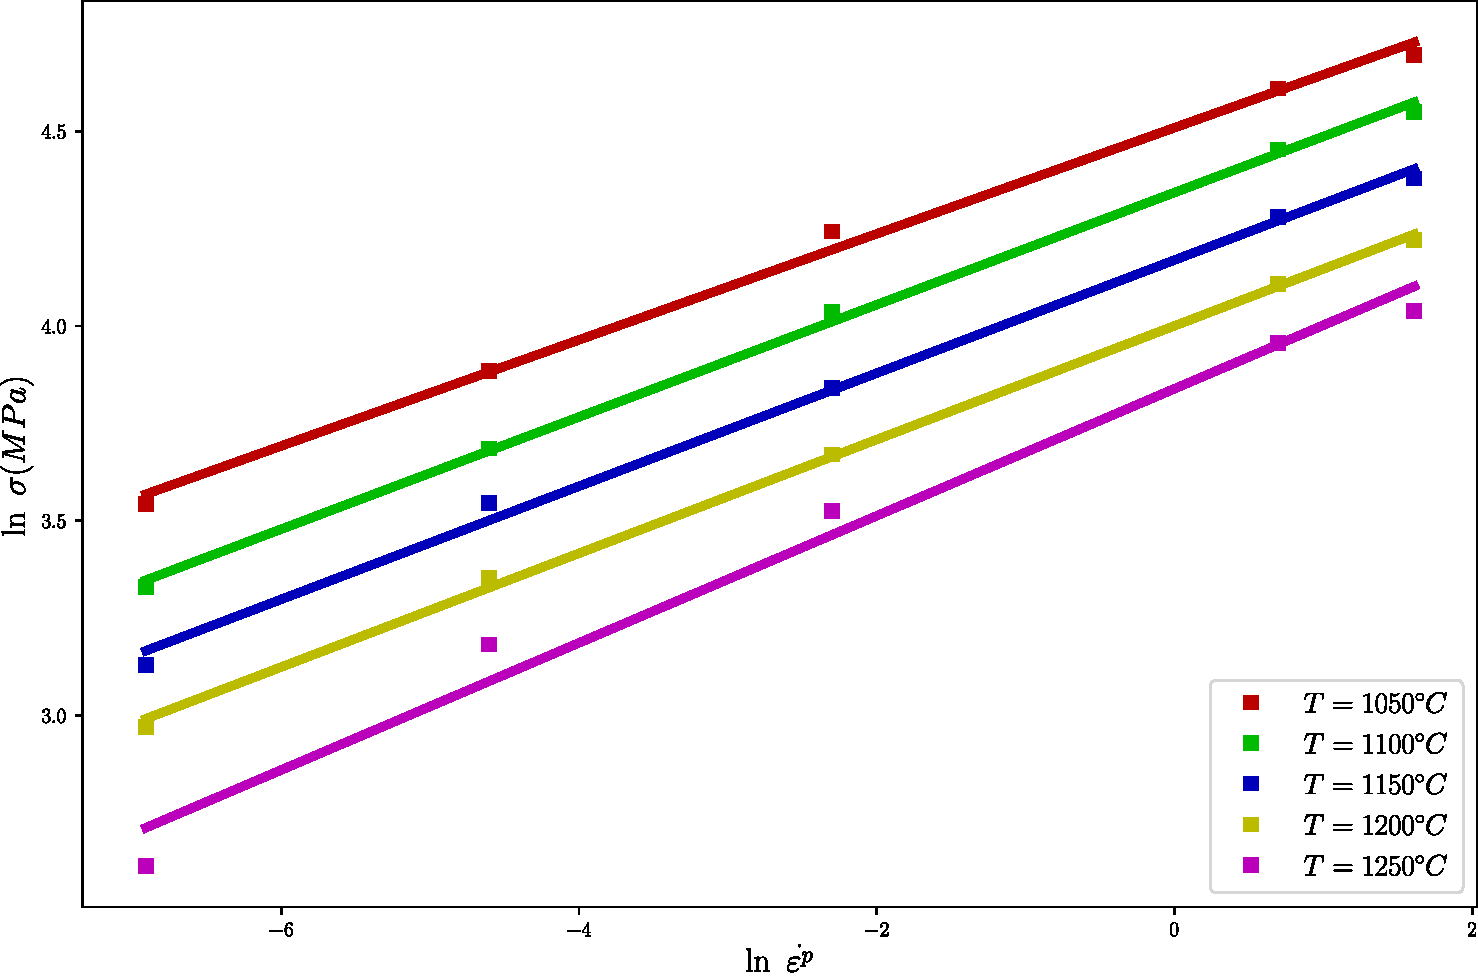
\includegraphics[width=0.9\columnwidth]{Figures/LnAlp}
\caption{Relationship between $\ln \sigma^y$ and $\ln \dot{\varepsilon}^p$}
\label{fig:LnAlp}
\end{figure}
\begin{figure}[!ht]
\centering
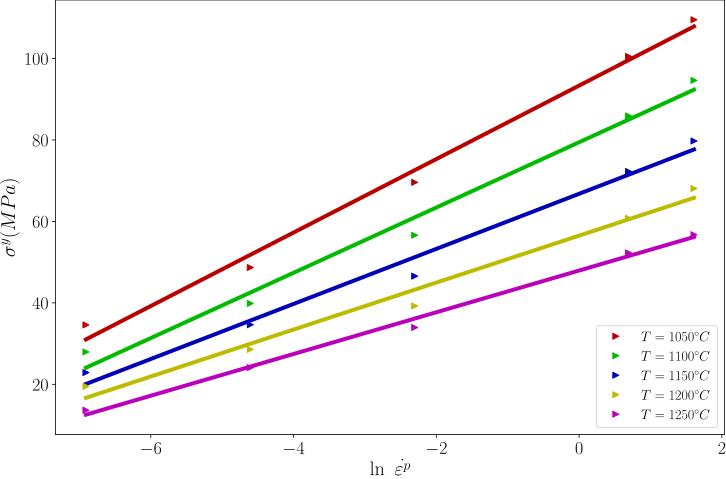
\includegraphics[width=0.9\columnwidth]{Figures/LnSinhE0}
\caption{Relationship between $\sigma^y$ and $\ln \dot{\varepsilon}^p$}
\label{fig:LnSinhE0}
\end{figure}
The values of those parameters are therefore equal to $n_1=6.78177$ and $\beta=0.150563$ ($\alpha=\beta/n_1 = 0.0222011$).
From Equation (\ref{eq:ARmodel}), the following relationship can be obtained:
\begin{equation}
\label{eq:lnSinh}
\ln\sinh(\alpha\sigma^y) = \frac{1}{n_2}\ln \mdot\varepsilon^p  -  \frac{1}{n_2}\ln A_3 + \frac{1}{n_2} \frac{Q}{RT}
\end{equation}
By applying the chain derivative rule, we get the following relationship to calculate the energy activation coefficient $Q$.
\begin{equation}
\label{eq:parQ}
Q = R\left[\frac{\partial \ln \mdot\varepsilon^p}{\partial \ln [\sinh(\alpha\sigma^y)]}\right]_{T}\left[\frac{\partial \ln [\sinh(\alpha\sigma^y)]}{\partial (1/T)}\right]_{\mdot\varepsilon^p}= Rn_2\frac{d\left\{\ln\left[\sinh(\alpha\sigma^y)\right]\right\}}{d(1/T)}
\end{equation}
From Equation (\ref{eq:lnSinh}) and Equation (\ref{eq:parQ}) we can deduce the parameters $n_2 $ and $Q $ from the slopes of the functions $\ln \sinh(\alpha\sigma^y) = f(\ln \dot{\varepsilon}^p)$ and $\ln \sinh(\alpha\sigma^y) = g(1/T)$ as shown in Figure \ref{fig:LnSinhE} and Figure \ref{fig:LnSinhT}. Thus those values are $4.94273$ and $437.385\ KJ.mol^{-1}$ respectively.
\begin{figure}[!ht]
\centering
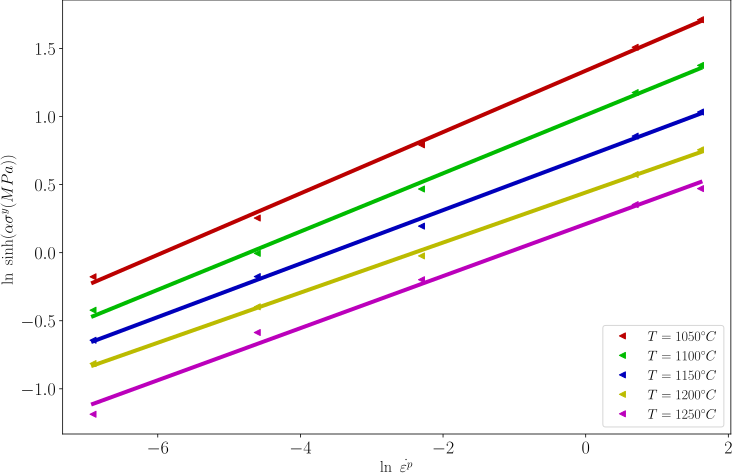
\includegraphics[width=0.9\columnwidth]{Figures/LnSinhE}
\caption{Relationship between $\ln \sinh(\alpha\sigma^y) $ and $\ln \dot{\varepsilon}^p$}
\label{fig:LnSinhE}
\end{figure}
\begin{figure}[!ht]
\centering
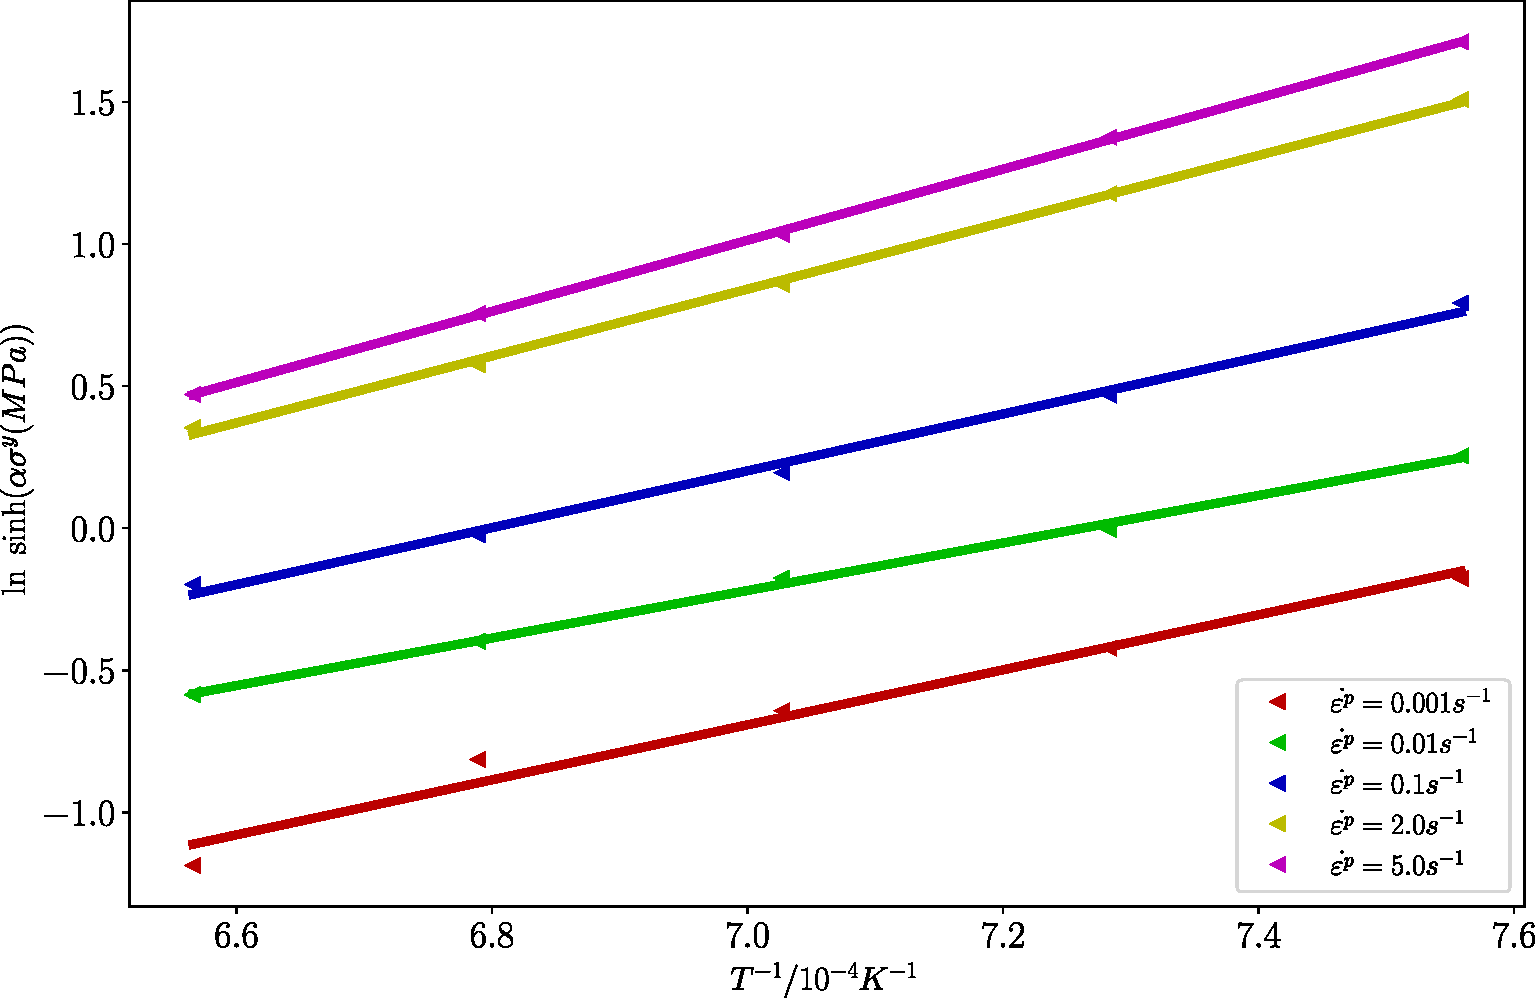
\includegraphics[width=0.9\columnwidth]{Figures/LnSinhT}
\caption{Relationship between $\ln \sinh(\alpha\sigma^y) $ and $1/T$}
\label{fig:LnSinhT}
\end{figure}
As these coefficients are calculated for a single strain value as example, it is possible to take into account their dependence on all strain values. Hence the need to find a function for each coefficient for all temperatures and strains. Figure  \ref{fig:ARparameters} shows the relationships between $\alpha$, $Q$, $n_2$, $\ln A$ and true strain $\varepsilon^p$ for AISI P20 alloy using leasquare method. For each parameter (whose strain dependant expressions are given by Equations \ref{eq:alpha}, \ref{eq:Q}, \ref{eq:n} and \ref{eq:lnA}), the values of constants are summarized in Table \ref{tab: ARparameters}. Figure \ref{fig:iCorrelationAR} is the comparison of predicted values of AR model and experimental values where the correlaton is good. The gap between experimental and prediction is small. But for the strain rate $\mdot\varepsilon^p = 0.01\ \text{s}^{-1}$ and for the two low temperatures values, the AR model is not able to predict the softening.
\begin{equation}
\label{eq:alpha}
\alpha(\varepsilon^p) = \alpha_0 + \alpha_1\varepsilon^{{p^1}} + \alpha_2\varepsilon^{p^2} + \alpha_3\varepsilon^{p^3} + \alpha_4\varepsilon^{p^4} + \alpha_5\varepsilon^{p^5} + \alpha_6\varepsilon^{p^6}
\end{equation}
\begin{equation}
\label{eq:Q}
Q(\varepsilon^p) = Q_0 + Q_1\varepsilon^{{p^1}} + Q_2\varepsilon^{p^2} + Q_3\varepsilon^{p^3} + Q_4\varepsilon^{p^4} + Q_5\varepsilon^{p^5} + Q_6\varepsilon^{p^6}
\end{equation}
\begin{equation}
\label{eq:n}
n_2(\varepsilon^p) = n_{20} + n_{21}\varepsilon^{{p^1}} + n_{22}\varepsilon^{p^2} + n_{23}\varepsilon^{p^3} + n_{24}\varepsilon^{p^4} + n_{25}\varepsilon^{p^5} + n_{26}\varepsilon^{p^6}
\end{equation}
\begin{equation}
\label{eq:lnA}
\ln A(\varepsilon^p) = \ln A_0 + \ln A_1\varepsilon^{{p^1}} + \ln A_2\varepsilon^{p^2} + \ln A_3\varepsilon^{p^3} + \ln A_4\varepsilon^{p^4} + \ln A_5\varepsilon^{p^5} + \ln A_6\varepsilon^{p^6}
\end{equation}
\begin{figure}[!ht]
\centering
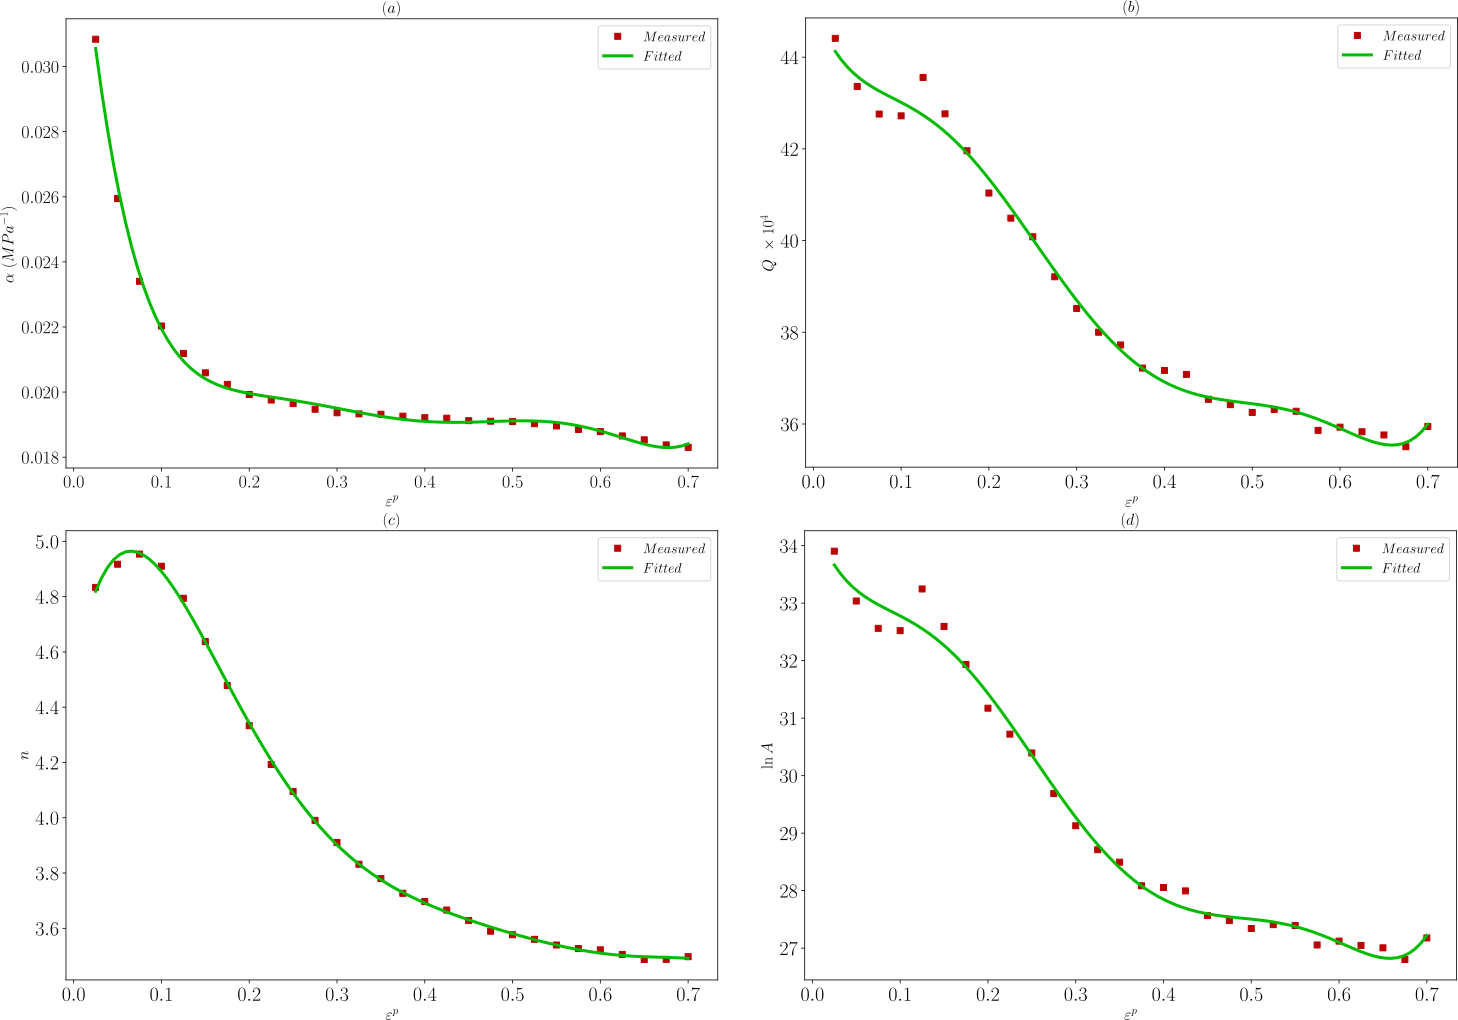
\includegraphics[width=1.02\columnwidth]{Figures/ARparameters}
\caption{Relationships between $\alpha$ (a)  , $Q$ (b) , $n_2$ (c)  and $lnA$ (d)  with the plastic strain $\varepsilon^p$ by polynomial functions}
\label{fig:ARparameters}
\end{figure}
\begin{table}[h!]
\centering{}
\caption{Parameters' constants of Arrhenius Model}
\begin{tabular}{lllll}
\hline
&					  &				      &				        &\\
Parameters&$\alpha$   &$Q (MJ.mol^{-1})$ &$n_2$                &$\ln A$\\
&					  &				      &				        &\\
\hline
&$\alpha_0 = 0.03702$ & $Q_0 = 0.454825$  & $n_{20} = 4.49273$  & $\ln A_0 = 34.7431$\\
&$\alpha_1 =-0.301107$& $Q_1 = -0.450492$ & $n_{21}=15.2803$    & $\ln A_1 =-36.826$\\
&$\alpha_2 = 2.19877$ & $Q_2=4.76922 $    & $n_{22} =-170.126$  & $\ln A_2 =393.423$\\
Values&$\alpha_3=-8.30819$&$Q_3 =-31.6016$& $n_{23} =651.241$   & $\ln A_3 =-2611.42$\\
&$\alpha_4 = 16.823$  & $Q_4 = 89.8821$   & $n_{24} =-1225.15$  & $\ln A_4 =7436.98$\\
&$\alpha_5 =-17.2732$ & $Q_5 =-113.829$   & $n_{25} =1143.54$   & $\ln A_5 =-9426.54$\\
&$\alpha_6 =7.04342$  & $Q_6 = 53.3699$   & $n_{26} =-423.066$  & $\ln A_6 =4422.49$\\
\hline
\label{tab: ARparameters}
\end{tabular}
\end{table}
\begin{figure}[!ht]
\centering
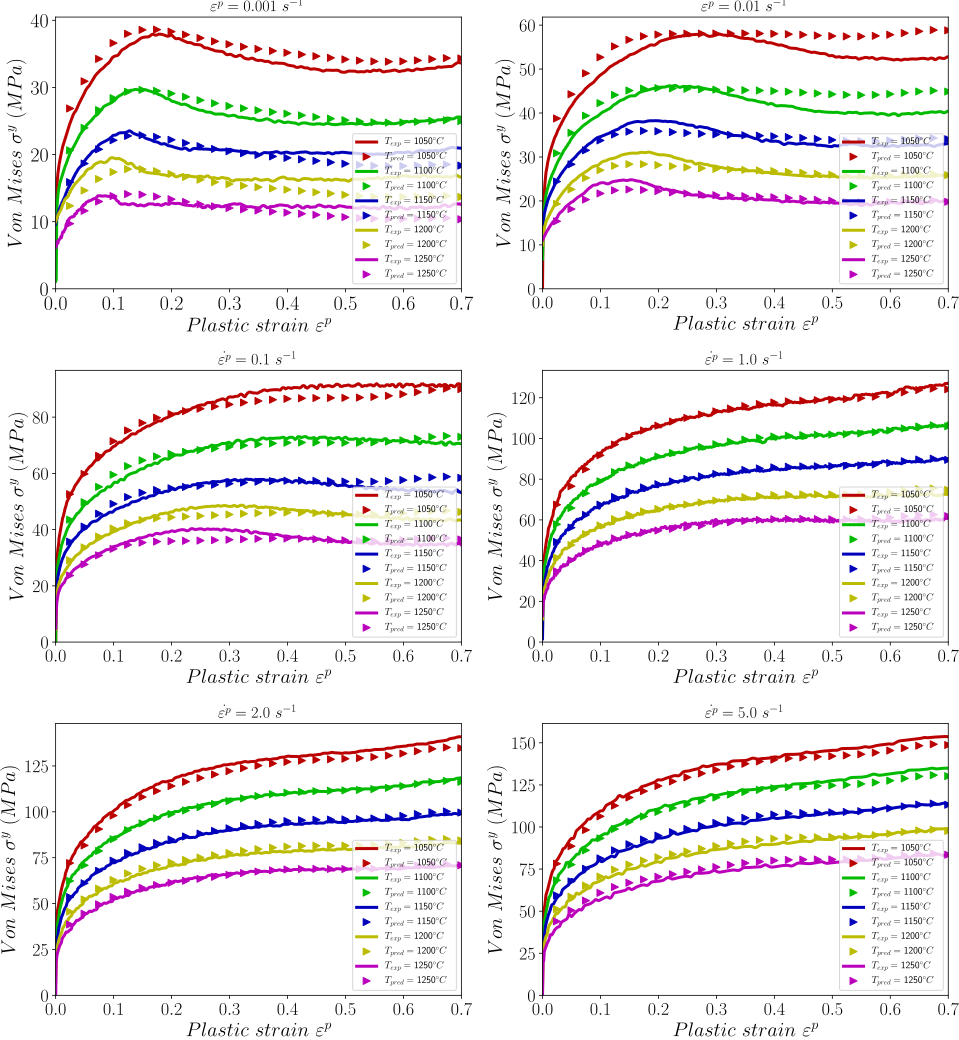
\includegraphics[width=1.02\columnwidth]
{Figures/CompExpAR}
\caption{Comparison between the experimental and predicted flow stresses by AR model}
\label{fig:iCorrelationAR}
\end{figure}
\FloatBarrier
%-------------------------------------------------------------------------
\subsection{PTM model\label{sec:ProposedModel}}
%--------------------------------------------------------------------------
The PTM model is a generalized formulation of the MZA model. Indeed, the shortcomings of the MZA model are taken into account in this formulation, which makes the model flexible for any type of studied material as it does not require a limited number of parameters. The intrinsic functions of the model, which are the polynomial type functions, will determine the parameters of the model according to the degree of the polynomial, which provides a good fit for each function. The equation describing the PTM model is therefore given by.
\begin{equation}
\label{eq:PTM-model}
\sigma^y(\varepsilon^p,\mdot\varepsilon^p,T) = \left(\sum_{i=0}^{q}{A_i\varepsilon^{p^i}}\right) \exp\left[\left(\sum_{j=0}^{r}{B_j\varepsilon^{p^j}}\right)\left(T-T_0\right) + \left(\sum_{k=0}^{s}\left(\sum_{l=0}^{t}{C_k^l\varepsilon^{p^l}} \right)\left(T-T_0\right)^k \right)\ln\left( \frac{\mdot\varepsilon^p}{\mdot{\varepsilon}_0}\right)\right]
\end{equation}
where $A_i, B_j, C_k^l$ are the parameters (Table \ref{tab:PTM-parameters}) of the model to be identified using the procedure proposed in  \cite{TizeMha-2022}. Quantities $q$, $r$, $s$ and $t$ define the degree of the polynomials used to describe the behavior of the material. The larger these quantities are, the more parameters need to be identified for the PTM model.
The determination of the parameters of this model are calculated thanks to the LMFIT Python library \cite{Newville-2016} and for more details about this model  we invite the reader to read our previous work \cite{TizeMha-2022}. Thus all the parametrers of this model are calcuted with $q=5$, $r=5$, $s=1$ and $t=5$.

Comparison of predicted values of the PTM model and experimental values is shown in Figure \ref{fig:iCorrelationPTM}. The PTM model is suitable to describe the flow behavior of AISI P20 steel, but for the strain rate $\mdot\varepsilon^p = 0.1\ \text{s}^{-1}$ the prediction in not quite good. The deviation between the predicted values and the experimental values is relatively good.
\begin{table}[!h]
\centering{}
\caption{Parameters of PTM model\label{tab:PTM-parameters}}
\begin{tabular}{cc}
\hline
&   \\
Parameters &Values\\
&   \\
\hline
$A_0 (\text{MPa})$ & $62.314$ \\
$A_1 (\text{MPa})$ & $559.827$ \\
$A_2 (\text{MPa})$ & $-2160.03$ \\
$A_3 (\text{MPa})$ & $4641.94,$ \\
$A_4 (\text{MPa})$ & $-5193.06$ \\
$A_5 (\text{MPa})$ & $2379.1$ \\
$B_0 $   & $-0.0035805$\\
$B_1 $   & $0.00282334$ \\
$B_2 $   & $-0.00775301$\\
$B_3 $   & $0.0085135$ \\
$B_4 $   & $-0.00412815$\\
$C_0^0 $ & $0.148304$ \\
$C_0^1 $ & $-0.301958$ \\
$C_0^2 $ & $2.2706$ \\
$C_0^3 $ & $-5.33003$ \\
$C_0^4 $ & $5.48971$ \\
$C_0^5 $ & $-2.11566$\\
$C_1^0 $ & $-3.74842\ \times10^{-7}$\\
$C_1^1 $ & $0.00165233$\\
$C_1^2 $ & $-0.00270485$ \\
$C_1^3 $ & $-0.000483867$\\
$C_1^4 $ & $0.00174818$ \\
\hline
\end{tabular}
\end{table}
\begin{figure}[!ht]
\centering
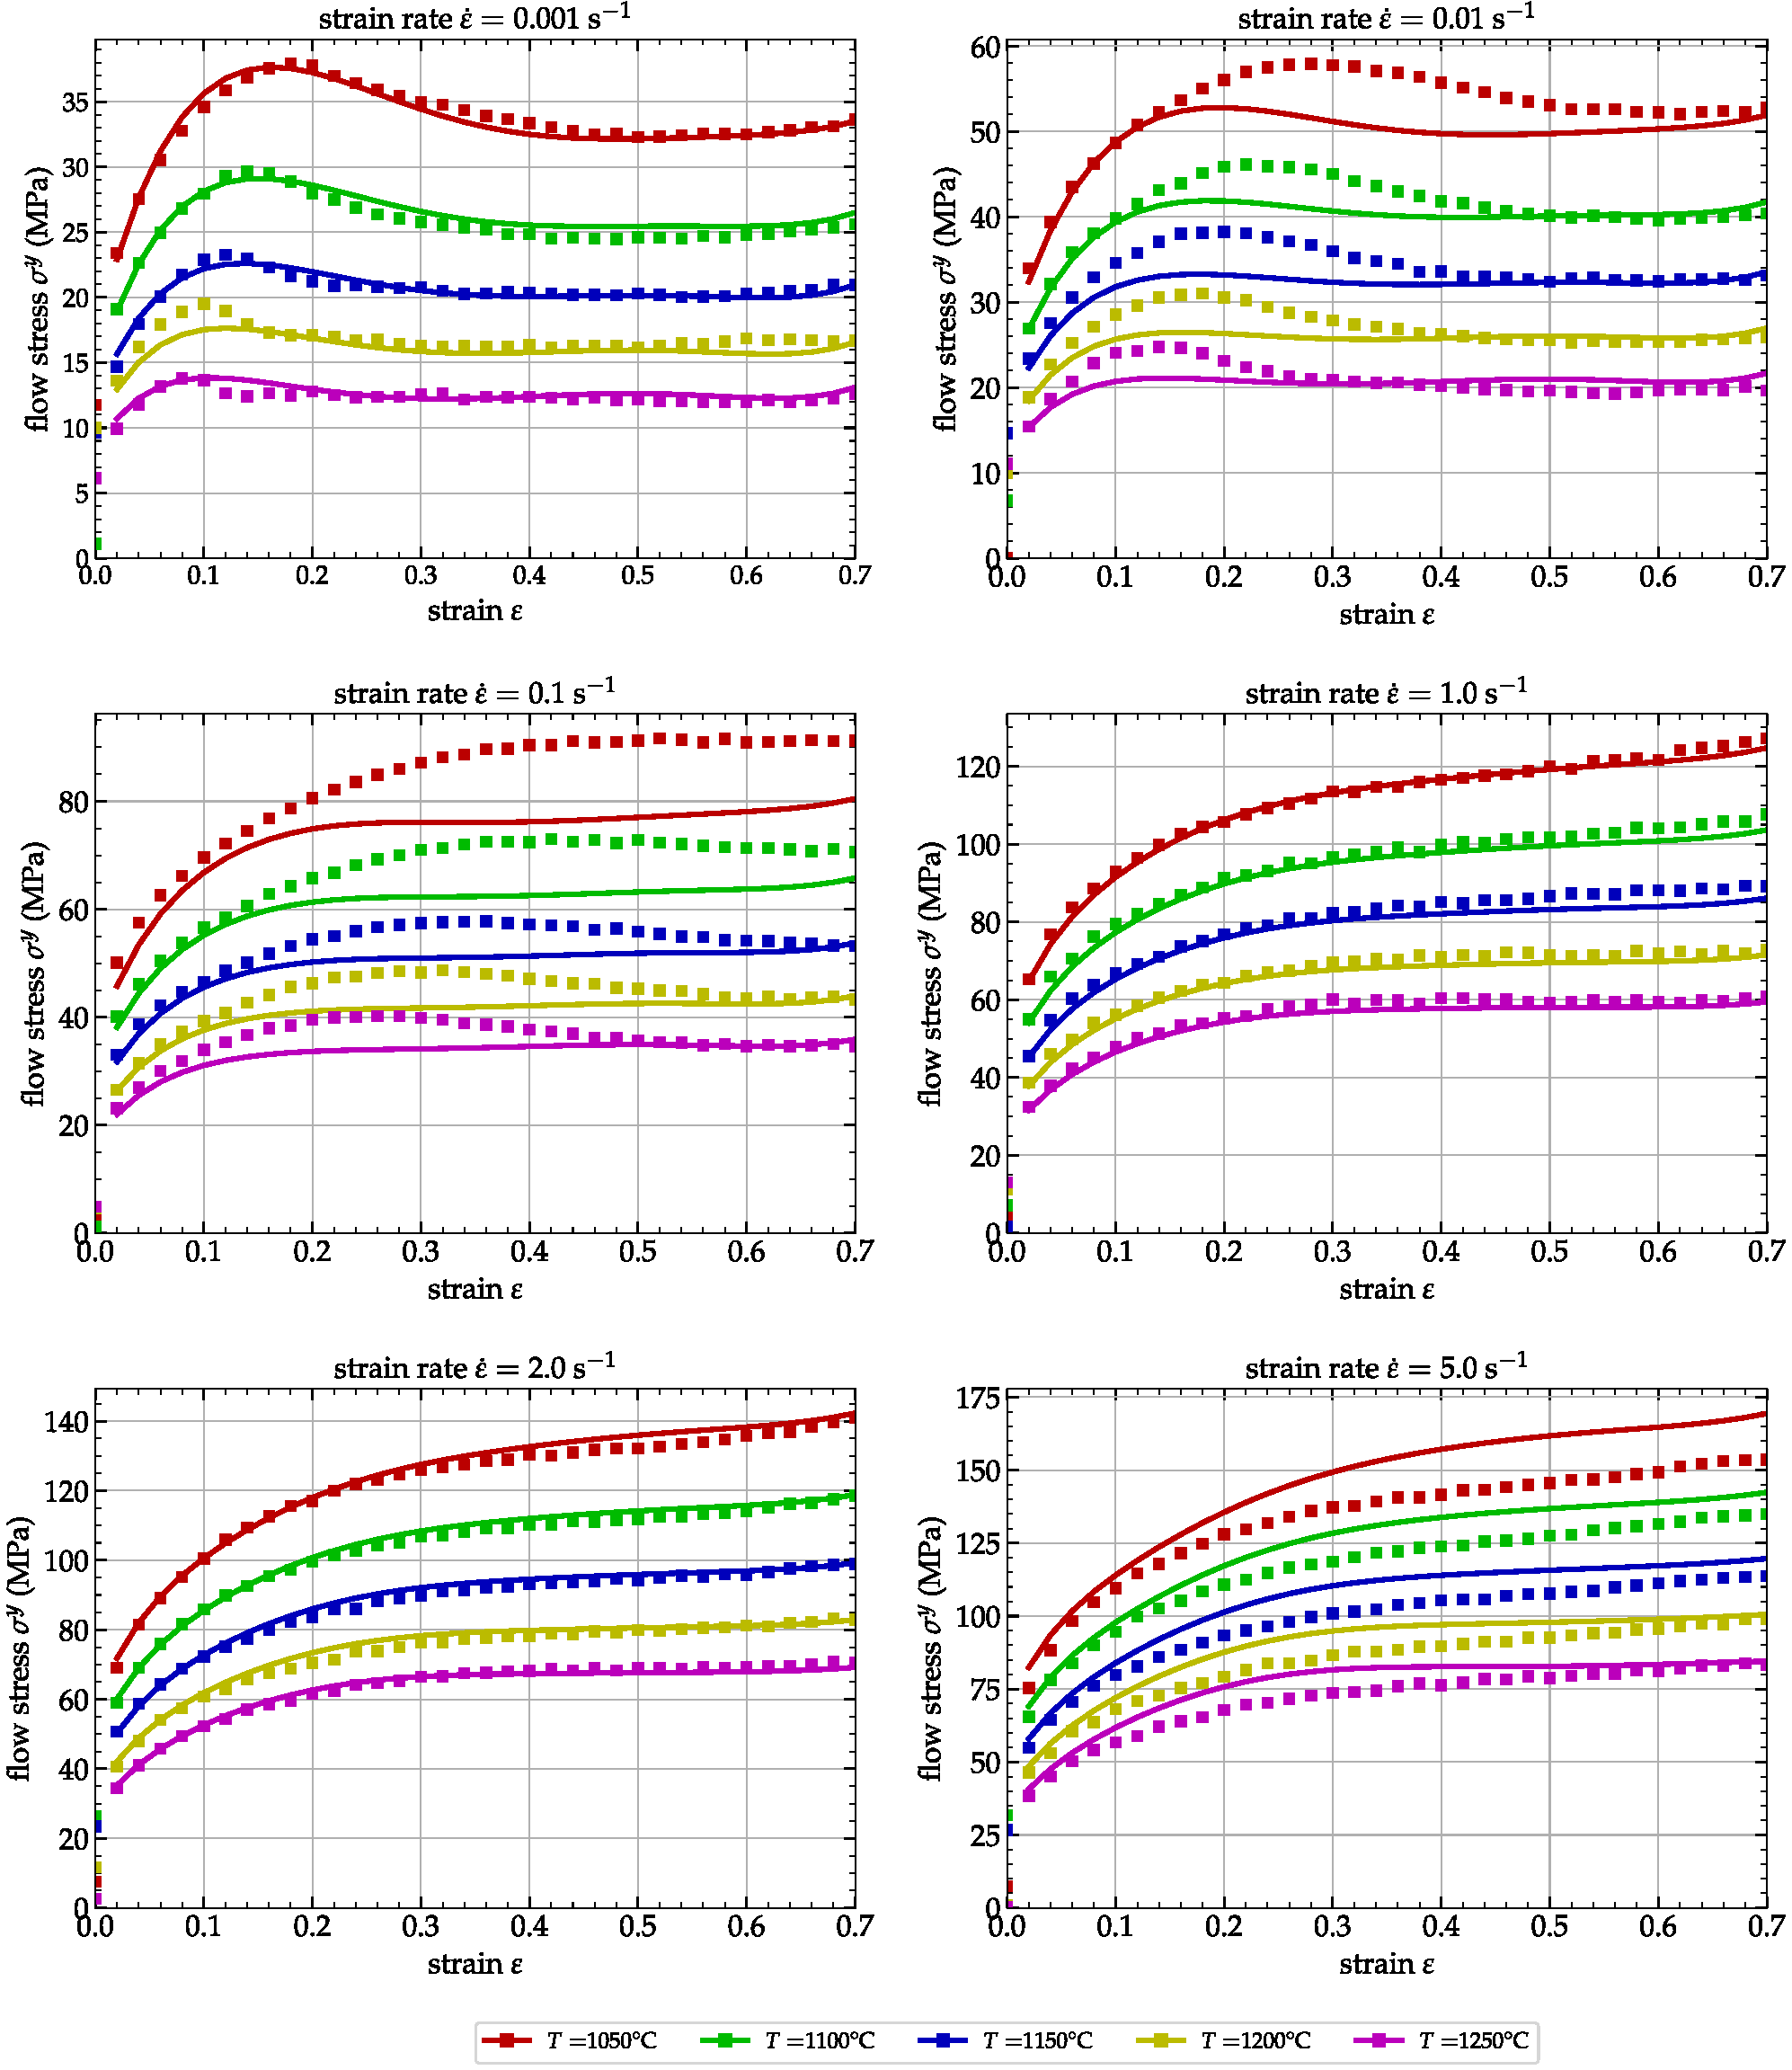
\includegraphics[width=1.02\columnwidth]
{Figures/CompExpPTM}
\caption{Comparison between the experimental and predicted flow stresses by PTM model }
\label{fig:iCorrelationPTM}
\end{figure}
\FloatBarrier

%-------------------------------------------------------------------------
\subsection{Artificial neural network model\label{sec:ANNmodel}}
%--------------------------------------------------------------------------
The Artificial Neural Network model (ANN) is a mathematical formulation widely used in many fields today for better prediction. It is a model based on the principle of minimisation where it improves from the progressive decrease of the error during the learning process. Typically an ANN model contains an input layer, an output layer and hidden layers. Each hidden layer is connected to the one before it and the one after it via neurons. Indeed, all neurons in the $k$ layer are connected to each neuron in the ($k+1$) layer. To each layer is added another parameter called bias. As said the principle of the ANN model is therefore based on the minimisation of the difference between the value obtained from the output of the network and the expected value.  Indeed, once the error is calculated, it is propagated back to the input layer in order to update the model parameters via the minimisation algorithms. In our case, the ADAM algorithm is used. The architecture of the network used in this study is shown in Figure \ref{fig:ANN-scheme-2HL}. After several tests of different types of network architecture, it was found that two hidden layers including $15$ neurons for the first hidden layer and $7$ for the second one gives the best prediction where the input layer is composed of three neurons ($\varepsilon^p$, $\mdot\varepsilon^p$, $T$) and the output layer is composed of a single neuron corresponding to the flow stress. The good performance of the model is found to be stable between $800$ and $1000$ epochs.

\begin{figure}[!ht]
\centering
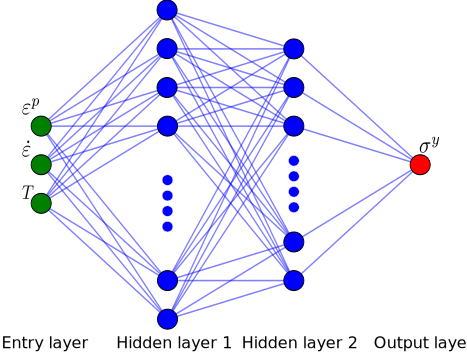
\includegraphics[width=0.7\columnwidth]
{Figures/ANN-scheme-2HL}
\caption{Multi-layer Artificial Neural Network architecture}
\label{fig:ANN-scheme-2HL}
\end{figure}

In this study $700$ of data were used; $80\%$ (560) are randomly selected for training and $20\%$ (140) for testing. Before learning, a normalisation of the data is required in order to have all data between $0$ and $1$. The Equation is widely used for normalization.
\begin{equation}
X_n = \frac{X - X_{min}}{X_{max} - X_{min}}
\end{equation}
Where $X$ is the orginal data ($\varepsilon^p$, $\log(\mdot\varepsilon^p/\varepsilon_0$,  $T$, $\sigma^y$), $X_{min}$ and $X_{max}$ are the minimum and maximum values of $X$ respectively. $X_n$ is the normalized data of the corresponding $X$. The trained model once tested can be used to predict the behavior of the AISI P20 alloy. Figure \ref{fig:iCorrelationANN} show a comparison between the predicted flow stresses from ANN model and measured data from hot compression test. As shown from this figures, the correlation between the experimental and the ANN prediction based is very good over the full range of data and the predicted data can well track the hardening and softening regions of the hot deforming material. Therefore, the ANN model can be used to simulate the hot deformation of this type of alloy. This was not necessarily the case with the analytical models. The performance of this prediction will be much more appreciated when it comes to testing its ability to predict data that has not been used in either the training or the test data, but rather a full-fledged trial that we wish to validate the ANN prediction by experimental. This validation will be done both with a strain rate between and outside of those used for the training step.
\begin{figure}[!ht]
\centering
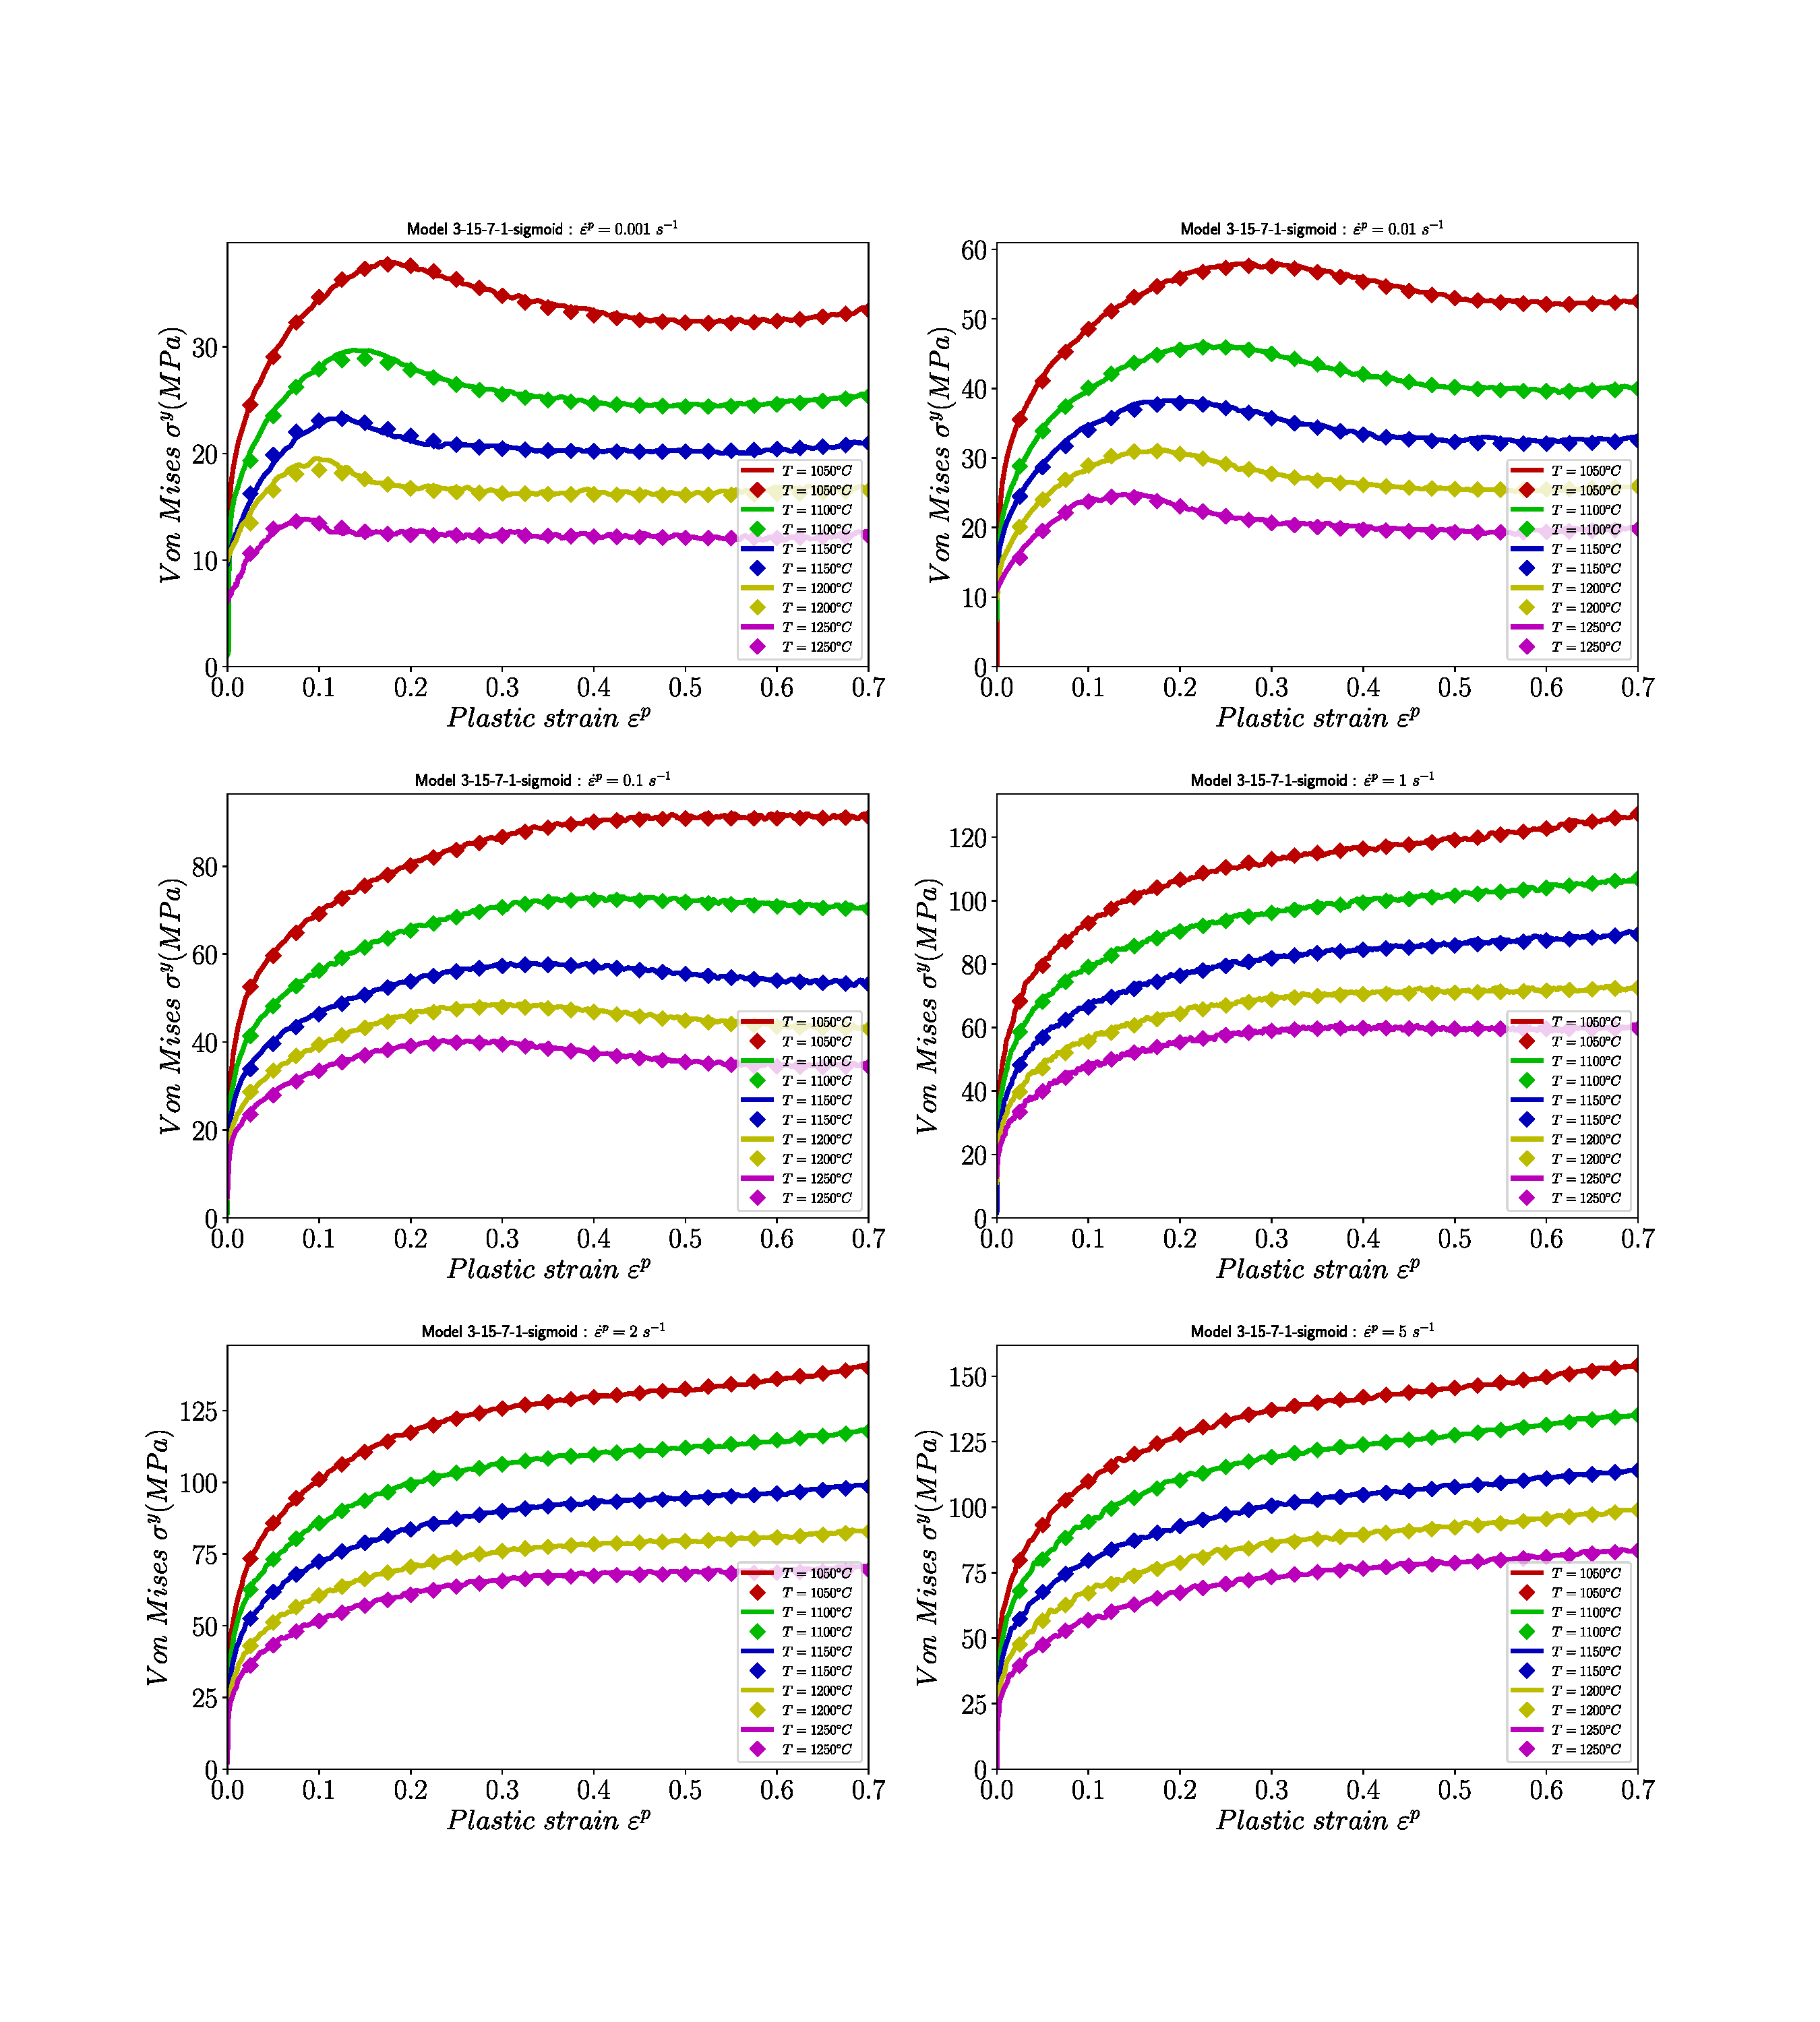
\includegraphics[width=1\columnwidth]
{Figures/CompExpANN}
\caption{Comparison between the experimental and predicted flow stresses by ANN model }
\label{fig:iCorrelationANN}
\end{figure}
\FloatBarrier
%-------------------------------------------------------------------------
\subsection{Comparison of analytical and ANN models\label{sec:Comparison}}
%--------------------------------------------------------------------------
\begin{figure}[!ht]
\centering
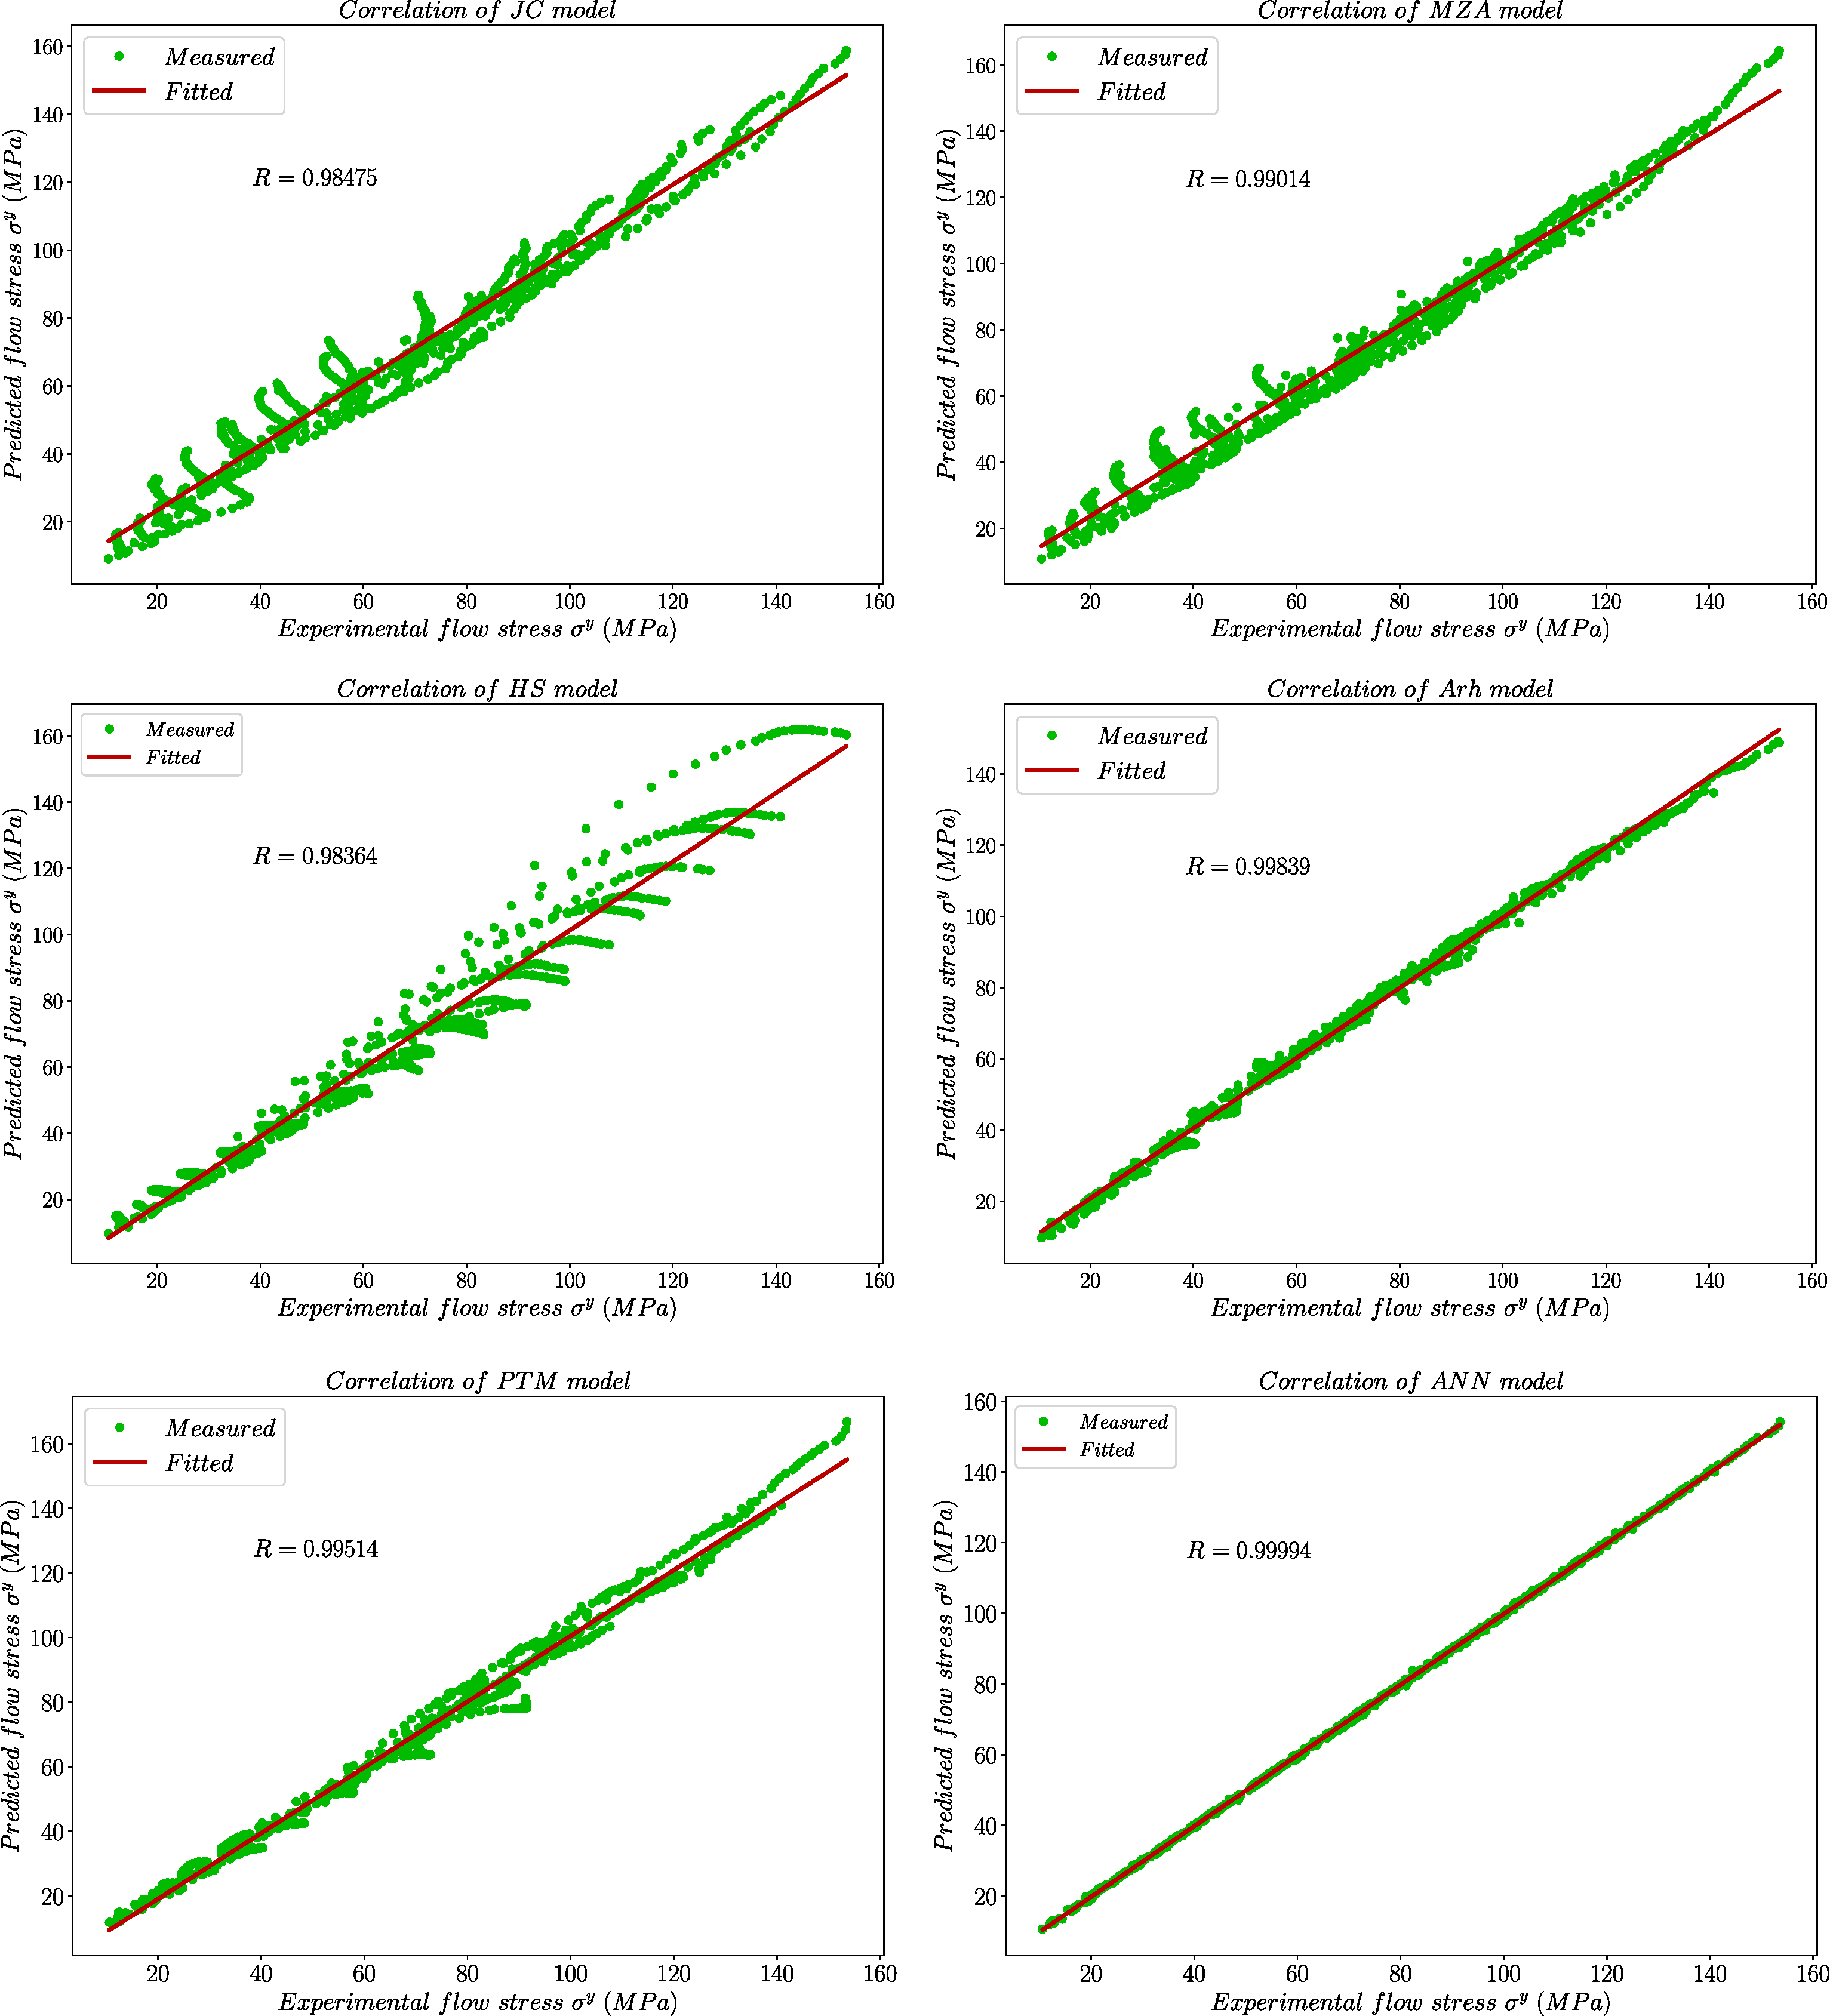
\includegraphics[width=1.02\columnwidth]
{Figures/Correlation}
\caption{Correlation coefficient ($R$) of models developed}
\label{fig:Correlation}
\end{figure}
The accuracy and predictive ability of both analytical and ANN models are generally assessed by some coefficients such as the correlation coefficient ($R$) (Equation (\ref{eq:R-expression})), Average Absolute Relative Error ($\AARE$ generally known as $\AARE$) (Equation (\ref{eq:AARE-expression})) and Root Mean Square Error ($\RMSE$) (Equation (\ref{eq:RMSE-expression})).
\begin{equation}
\label{eq:R-expression}
\R(\%) = \frac{\displaystyle\sum_{i=1}^{N}{\left(E_i - \overline{E}\right)\left(P_i - \overline{P}\right)}}{\sqrt{\displaystyle\sum_{i=1}^{N}\left(E_i - \overline{E}\right)^2 .\displaystyle\sum_{i=1}^{N}\left(P_i - \overline{P}\right)^2}}\times 100
\end{equation}
\begin{equation}
\label{eq:AARE-expression}
\AARE(\%) = \frac{1}{N}\displaystyle\sum_{i=1}^{N} \displaystyle\left\lvert\frac{E_i- P_i}{E_i} \right\rvert\times 100
\end{equation}
\begin{equation}
\label{eq:RMSE-expression}
\RMSE (\text{MPa}) = \sqrt{\frac{1}{N} \displaystyle\sum_{i=1}^{N} \left(E_i - P_i\right)^2}
\end{equation}
Where $E_i$ is the experimental value and $P_i$ is the predicted value of the constitutive law (phenomenological and ANN models), $\overline{E}$ and $\overline{P}$ are the mean values of the experimental and predicted values, respectively.

The correlation coefficient $R$ is generally used to show the degree of linearity between the experimental and predicted values. The model sometimes tends to be biased towards low and high values. Therefore, a good (high) value of $R$ does not necessarily mean a good prediction of the model but simply establishes a good linearity correlation between the experiment and the prediction \cite{Phaniraj-2003}. On the other hand, other coefficients ($\AARE$ and $\RMSE$) are used to estimate the predictive capacity of the model because they are considered unbiased as well as for low and high values. Indeed, they verify the predictability of a model term by term comparison of the relative error in relation to the real value of the variable \cite{Srinivasulu-2006}. Thus the correlation coefficients $R$ for JC, MZA, HS, Arhenius, proposed and ANN models are $0.98475$,  $0.99014$,  $0.98364$, $0.99839$, $0.99514$, and $0.99994$ respectively as shown on Figure \ref{fig:Correlation}. These results show that all models have a relatively good coefficient; this does not guarantee the validation of the prediction of these models. Hence the need to calculate the other two coefficients. All coefficients for evaluating the high-temperature flow stress prediction capability of the AISI P20 alloy for all models presented in this work are summarized in the Table \ref{tab:Coefsparams}.

From this table, it can be seen that the ANN model has a good prediction than the analytical models. All this shows sufficiently that the ANN model is more effective in describing the behavior of the AISI P20 alloy for high temperature deformation. This efficiency will therefore be validated on tests at two different selected strain rates. One between the minimum and the maximum strain rates used during identification or training for ANN model and another one outside higher than the maximum strain rate. This will validate the interpolation and extrapolation capability of phenomenological and ANN models. The prediction results should lead to a better interpolation and extrapolation capability of the ANN model than phenomenological models as shown by identification. Another thing to be analysed from this table is the link between the values of the correlation coefficient $R$ and the values of $\AARE$ and $\RMSE$. Indeed, as mentioned above, the $R$ coefficient does not necessarily mean a good prediction of the model but a good relationship of linearity between the experiment and the prediction. To ensure a good prediction of the model, it is necessary to add to $R$, the values of $\AARE$. From that table it can be seen the values of the coefficients $R$ are $99.014\%$, $98.364\%$, for $\AARE$ are $11.13020\%$ and $8.15103\%$ and those of $\RMSE$ are $5.35079\ \text{MPa}$, and $6.45287\ \text{MPa}$ respectively for the MZA model and the HS model. This seems contradictory when the $R$ of HS is smaller than that of MZA, whereas for the $\AARE$ and $\RMSE$ values it is the opposite case. This simply means that the HS model has a good prediction compared to the MZA model whereas in the framework of the linear correlation between the experiment and the prediction the MZA model makes it better. All this can be seen from the identification curves where we can observe the HS curves (Figure \ref{fig:iCorrelationHS}) are indeed closer to the experimental than those of MZA (Figure \ref{fig:iCorrelationMZA}) while the points are scattered for HS model on the correlation curve (Figure \ref{fig:Correlation}). This validates the analysis made by \cite{Phaniraj-2003, Srinivasulu-2006}.

\begin{table}[h!]
\centering{}
\caption{Accurary coefficients of the developped models}
\begin{tabular}{lcccccc}
\hline
&		&		&         &             &		   &		  		\\
Coefficients&JC  & MZA  &HS  & Arhenius      & PTM  &ANN  		    \\
&				&				&         &             &		   &\\
\hline
$R(\%)$&$98.4745$&$99.0141$&$98.5682$&$99.839$& $99.5137$&$99.9994$ \\
$\AARE(\%)$&$11.1667$&$11.13020$&$8.15103$&$3.30677$&$4.19549$&$0.81094$   \\
$\RMSE(\text{MPa})$&$6.30298$&$5.35079$&$6.45287$&$2.03275$&$3.59027$&$0.55158$\\
\hline
\label{tab:Coefsparams}
\end{tabular}
\end{table}

%-------------------------------------------------------------------------
\section{Interpolation and extrapolation capability of phenomenological and ANN models \label{sec:inExtrapolation}}
%--------------------------------------------------------------------------
In this section we wish to test the performance of each identified model data interpolating and extrapolating data. Indeed, out of the $6$ strain rates used, one strain rate is voluntarily removed (while keeping the same values of strains and temperatures used for the development of the phenomenological and ANN models) so that it is inside or outside the other $5$ strain rates. For the strain rate which is between the minimum and the maximum of the $5$ other strain rates, we will thus test the capacity of each model to interpolate the data and for the one which is out of the $5$ other strain rates, the extrapolation capacity of the model is therefore validated. The validation procedure is as follows: $5$ strain rates are used to re-identify each model and once identified, it is used to predict the flow stress for the strain rate chosen for both interpolation and extrapolation. Validation is done with real data. The following subsections will highlight this procedure.
\subsection{Interpolation validation}
For the validation of the interpolation, the chosen strain rate is $\mdot\varepsilon^p = 1.0\ \text{s}^{-1}$ and those used for identification (training for ANN) are $\mdot\varepsilon^p = 0.001\ \text{s}^{-1}$ , $\mdot\varepsilon^p = 0.01\ \text{s}^{-1}$ , $\mdot\varepsilon^p = 0.1\ \text{s}^{-1}$, $\mdot\varepsilon^p = 2.0\ \text{s}^{-1}$  and $\mdot\varepsilon^p = 5.0\ \text{s}^{-1}$. The Figure \ref{fig:inCombinaison} shows the comparison between the predictions of the analytical and ANN models and the experiment. It appears from these Figures that all models have relatively good predictions but the ANN model remains the best because the value of its $\AARE$ is $1.4\%$ while it is between $2.33\%$ and $6.13\%$ for the analytical models. This further shows the performance of the ANN model compared to the analytical models. All these results are summarized in Table \ref{tab:inValid}.
\begin{figure}[!ht]
\centering
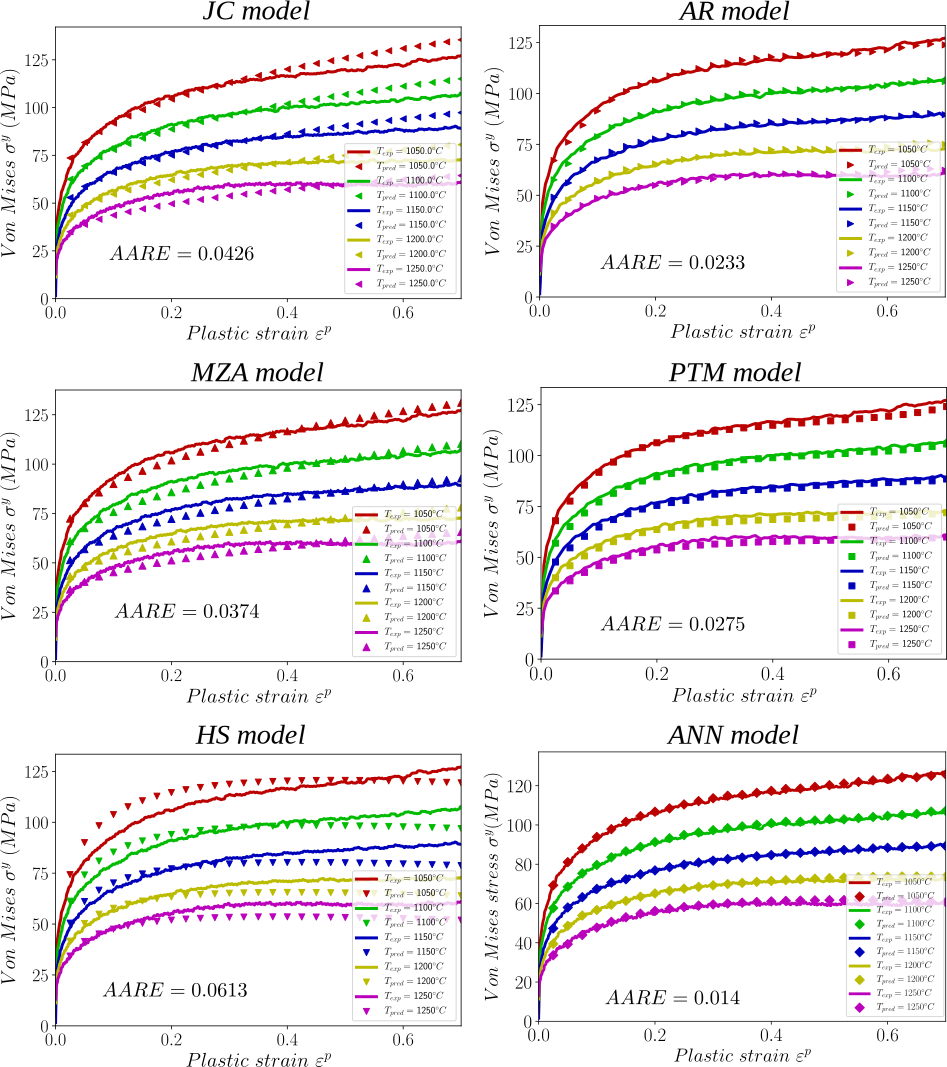
\includegraphics[width=1.02\columnwidth]
{Figures/inCombinaison}
\caption{Comparison between the experimental and predicted flow stresses by ANN model for interpolation estimation}
\label{fig:inCombinaison}
\end{figure}
\begin{table}[h!]
\centering{}
\caption{Accuracy coefficients of interpolation}
\begin{tabular}{lcccccc}
\hline
&		&		&         &             &		   &	\\
Coefficients&JC  & MZA  &HS  & Arhenius      & PTM  &ANN \\
&				&				&         &             &	&\\
\hline
$R(\%)$&$99.0590$&$99.0821$&$97.6008$&$99.8417$& $99.8760$&$99.9439$  \\
$\AARE(\%)$&$4.2686$&$3.7440$&$6.1391$&$2.3321$&$2.7590$&$1.4018$   \\
$\RMSE(\text{MPa})$&$4.1923$&$3.1856$&$82.6956$&$2.29891$&$2.4632$&$1.0228$ \\
\hline
\label{tab:inValid}
\end{tabular}
\end{table}
\subsection{Extrapolation validation}
For the validation of the extrapolation, the chosen strain rate is $\mdot\varepsilon^p = 5.0\ \text{s}^{-1}$ and those used for identification (training for ANN) are $\mdot\varepsilon^p = 0.001\ \text{s}^{-1}$ , $\mdot\varepsilon^p = 0.01\ \text{s}^{-1}$ , $\mdot\varepsilon^p = 0.1\ \text{s}^{-1}$, $\mdot\varepsilon^p = 1.0\ \text{s}^{-1}$  and $\mdot\varepsilon^p = 2.0\ \text{s}^{-1}$. Figure \ref{fig:exCombinaison} shows the comparison between the predictions  and the experimental. Unlike interpolation, the predictions of the analytical models are not very good because the errors are between $3.2\%$ and $12.99\%$ while that of the ANN model is $1.74\%$. Again, the ANN model shows its ability to extrapolate data. This makes it possible to say that the ANN model remains the best tool to characterize the behavior of a material subjected to certain deformation conditions. It can also be noted that the Arhenius and the PTM models still have some ability to extrapolate because their $\AARE$ are respectively $ 3.2 \% $ and $ 3.8 \%$; which are acceptable.
\begin{table}[h!]
\centering{}
\caption{Accuracy coefficients of extrapolation}
\begin{tabular}{lcccccc}
\hline
&		&		&         &             &		   &	\\
Coefficients&JC  & MZA  &HS  & Arhenius      & PTM  &ANN \\
&				&				&         &             &	&\\
\hline
$R(\%)$&$99.2920$&$99.4879$&$93.9429$&$99.6870$& $99.7582$&$99.8047$\\
$\AARE(\%)$&$4.8988$&$3.4506$&$12.9939$&$3.2008$&$3.8845$&$1.7433$\\
$RMSE(\text{MPa})$&$5.0943$&$4.3048$&$116.517$&$3.7035$&$4.3915$&$1.2513$ \\
\hline
\label{tab:exValid}
\end{tabular}
\end{table}
\begin{figure}[!ht]
\centering
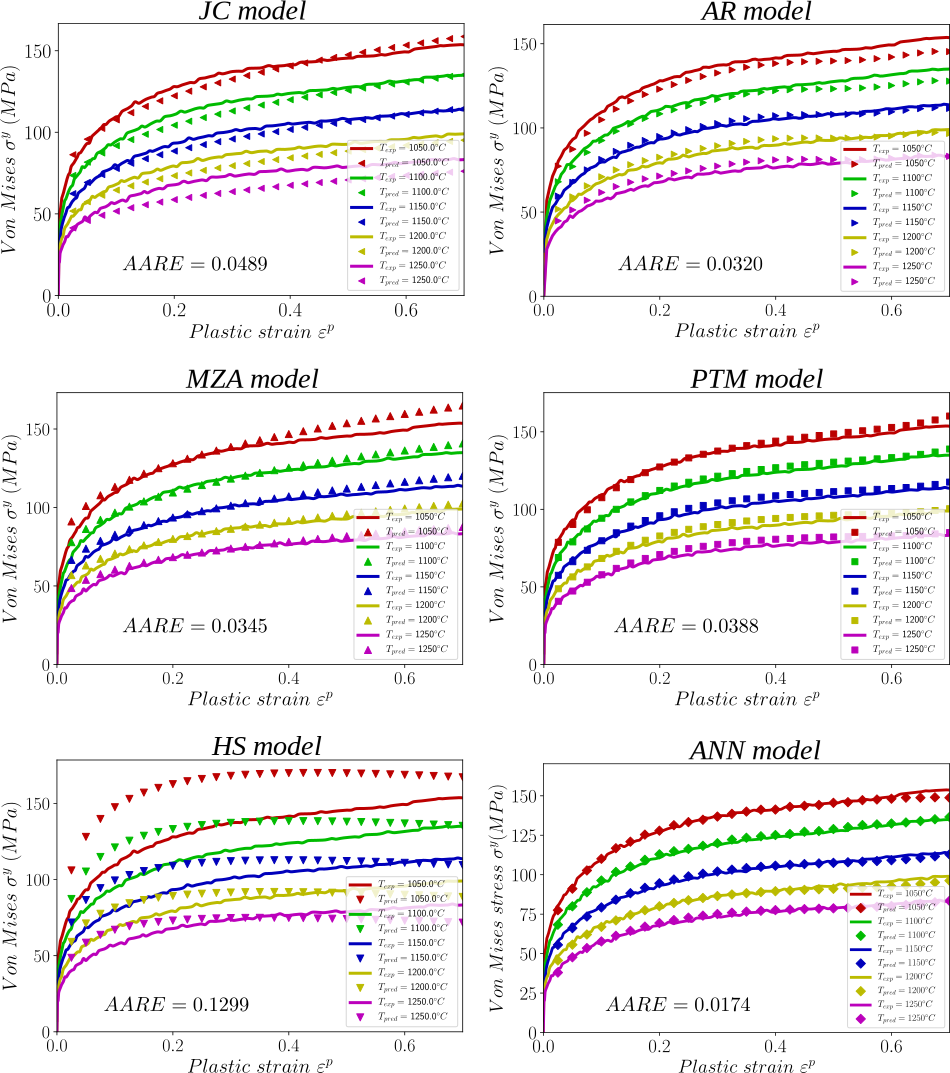
\includegraphics[width=0.91\columnwidth]
{Figures/exCombinaison}
\caption{Comparison between the experimental and predicted flow stresses by ANN model for extrapolation estimation}
\label{fig:exCombinaison}
\end{figure}
\FloatBarrier
%---------------------------------------------------------------------
\section{Conclusion \label{sec:Conclusion}}
Experiments were conducted on modified AISI P20 carbon alloy to study the applicability and predictive accuracy of five analytical models and one neural network model over a range of temperatures ($1050$°C - $1250$°C, strains ($0.025$ - $0.7$), strain rates ($0.001\ \text{s}^{-1}$ - $5\ \text{s}^{-1}$) and the following conclusions were drawn.
\begin{enumerate}
\item The flow stress increases with decreasing temperature and increasing strain rate due to the competitive occurrence of dynamic softening and strain hardening mechanisms.  The degree of DRX was discussed through the difference between the maximum and permanent stress, as well as the evolution of the microstructure which shows a partially complete DRX. At high strain rates it is difficult to visualise the DRX phenomenon on the flow curves due to the strain rate sensitivity of this phenomenon. A further study will focus on deep analysis of the microstructure of this steel alloy and its impact on mechanical properties.
\item Five analytical models have been identified on this alloy and a model based on neural networks. Among the analytical models, the JC, HS and MZA models proved inappropriate for analysing the behavior of this material whereas the PTM and AR models showed their capacity since they have a relatively acceptable error ($ 3.2 \% $ and $ 3.8 \%$). As for the ANN model, it is largely reliable that the analytical models to predict the competitiveness of AISI P20. Therefore it may be advisable to use the ANN model when conducting a study involving this alloy under these experimental conditions.
\item To test the performance of each model, a study is carried out to evaluate the interpolation and extrapolation capacity of the developed models. For the interpolation framework, all models have a good correlation with the experiment except the HS model but the ANN model shows a better correlation.  For extrapolation of the data, the analytical models do not show good predictive capacity compared to the ANN model which still shows good extrapolation capacity. This further confirms what was demonstrated during his identification.
\item As perspectives of this work, we will develop also an ANN model to characterize the microstructure in terms of DRX and phase formation such as fearrite, bainite and martensite as an example. This ANN model can therefore be compared to the most commonly used classical models such as the JMAK model. Therfore, this ANN model  will be implemented in FEM softwares such as Abaqus, Forge in order to validate it by doing a simulation.
\end{enumerate}
% \bibitem{}
\bibliographystyle{elsarticle-num}
\bibliography{Bibliography}
%\end{thebibliography}
\end{document}
\endinput

